\typeout{NT FILE DESIGN.tex}%
\chapter{Design}%
\label{ch:design}
\begin{quote}
\begin{flushright}
``\emph{Simplicity is the ultimate sophistication.}'' \\
\textbf{-- Leonardo Da Vinci}, polymath
\end{flushright}
\end{quote}

The previous survey motivates using a small, open-source, statically partitioned
hypervisor as the consolidation mechanism. We now translate those findings into
a concrete architecture for video-surveillance \glspl{uav} under tight \gls{swap-c}:
the \gls{sspfs}, a flight stack that leverages the Bao hypervisor so that
resource-intensive, non-critical streaming can coexist with safety-critical
flight control on consolidated hardware.
%
We begin by stating requirements and constraints for the target application, then
analyze the conventional split architecture and its drawbacks. We implement an
unsupervised single-platform baseline (\gls{uspfs}) to quantify consolidation
overheads, and subsequently deploy the supervised counterpart atop Bao
(\gls{sspfs}).
%
Next, we select the hardware (the \gls{uav} and the \gls{uavic}) and map these
components into the \gls{uspfs} and \gls{sspfs} designs. To support shared
\gls{pcie} devices across \glspl{vm}, we introduce a supervised mailbox
mechanism. We conclude by adapting the hardware mapping to constraints imposed
by the \gls{uavic} platform and the Bao hypervisor.

\section{Requirements and Constraints}
\label{sec:req-sec}

Video-surveillance missions require two capabilities: (i) geolocation control to
survey a designated area and (ii) image acquisition to gather pertinent
information about that region. Both can be achieved via \emph{offline} or
\emph{online} command methods, or a combination of the two~\cite{gugan2023path}.
%
In the \emph{offline} approach, the target area and the information to be
captured are well defined and can be specified \emph{a priori} to the
\gls{uav}~\cite{gugan2023path}. In cartographic applications, for example, the
\gls{uav} systematically scans the area to collect topographic
data~\cite{caroti_uav-borne_2017}; the vehicle can then operate fully
autonomously and store data locally~\cite{qgc-survey}.
%
The \emph{online} approach suits dynamic and unpredictable environments where
the area of interest and relevant cues are not fully
predefined~\cite{gugan2023path}. In rescue missions, target identification is
critical and requires active supervision by the
\gls{gcs}~\cite{mohsan2022towards}; the \gls{gcs} must be able to remotely
command the \gls{uav} and receive real-time feedback, including telemetry and
live video.
%
Given these demands, this work focuses on the online command mode, which imposes stricter operational requirements on both the platform and the software stack.

Table~\ref{tab:requirements} summarizes the requirements and constraints
considered in this thesis. Functional requirements include real-time telemetry
and command, video surveillance, autonomous flight control, and battery
operation. Technical requirements mandate fault-tolerant isolation between
components, minimal security overhead, and consolidation of flight-control and
companion functions on shared hardware. Functional constraints prioritize weight
minimization and bandwidth-efficient video transmission, while technical
constraints specify an open-source stack, wireless communications, and the use
of the Bao hypervisor for enforcement of isolation.


\begin{table}[t]
  \centering
  \caption{System requirements and constraints for the UAV flight stack}
  \label{tab:requirements}

  % ---- local-only tweaks (end at \endgroup) ----
  \begingroup
  \small % or \footnotesize if you need it smaller
  \setlength{\tabcolsep}{6pt}     % default ~6pt; lower for tighter columns
  \renewcommand{\arraystretch}{1.05} % slightly tighter rows

  \begin{tabularx}{\textwidth}{
    >{\raggedright\arraybackslash}p{0.20\textwidth}  % group label
    >{\raggedright\arraybackslash}X                   % Functional
    >{\raggedright\arraybackslash}X                   % Technical
  }
    \toprule
    \textbf{Categorization} & \textbf{Functional} & \textbf{Technical} \\
    \midrule
    \textbf{Requirements} &
    \begin{itemize}[leftmargin=*,nosep,topsep=0pt]
      \item Remote UAV command and geolocation in (soft) real time
      \item Real-time image acquisition
      \item Onboard flight-stabilization mechanisms
      \item Battery-powered flight autonomy
    \end{itemize}
    &
    \begin{itemize}[leftmargin=*,nosep,topsep=0pt]
      \item Fault tolerance: video compromise must not affect flight control
      \item Minimal added latency from security mechanisms
      \item Consolidation of flight and companion functions on a single hardware platform
    \end{itemize}
    \\
    \addlinespace[0.3em]
    \textbf{Constraints} &
    \begin{itemize}[leftmargin=*,nosep,topsep=0pt]
      \item Minimal weight to preserve flight autonomy
      \item Bandwidth-optimized video transmission
    \end{itemize}
    &
    \begin{itemize}[leftmargin=*,nosep,topsep=0pt]
      \item Open-source flight stack (e.g., PX4)
      \item Wireless control and image transmission
      \item Use of the Bao hypervisor for security and fault tolerance
    \end{itemize}
    \\
    \bottomrule
  \end{tabularx}
  \endgroup
  % ---- local-only tweaks end here ----
\end{table}

\section{System Architecture}
\label{sec:design-sysArch}

Figure~\ref{fig:uav-design-conv-sol-1} illustrates the conventional solution
(\glsxtrfull{umpfs}) for video surveillance, which separates concerns across two
nodes. The flight-controller hardware node manages flight-critical functions,
while the companion-computer node handles secondary and compute-intensive tasks
(e.g., collision avoidance, odometry, and video streaming to the \gls{gcs}).

\begin{figure}[!hbt]
  \centering
  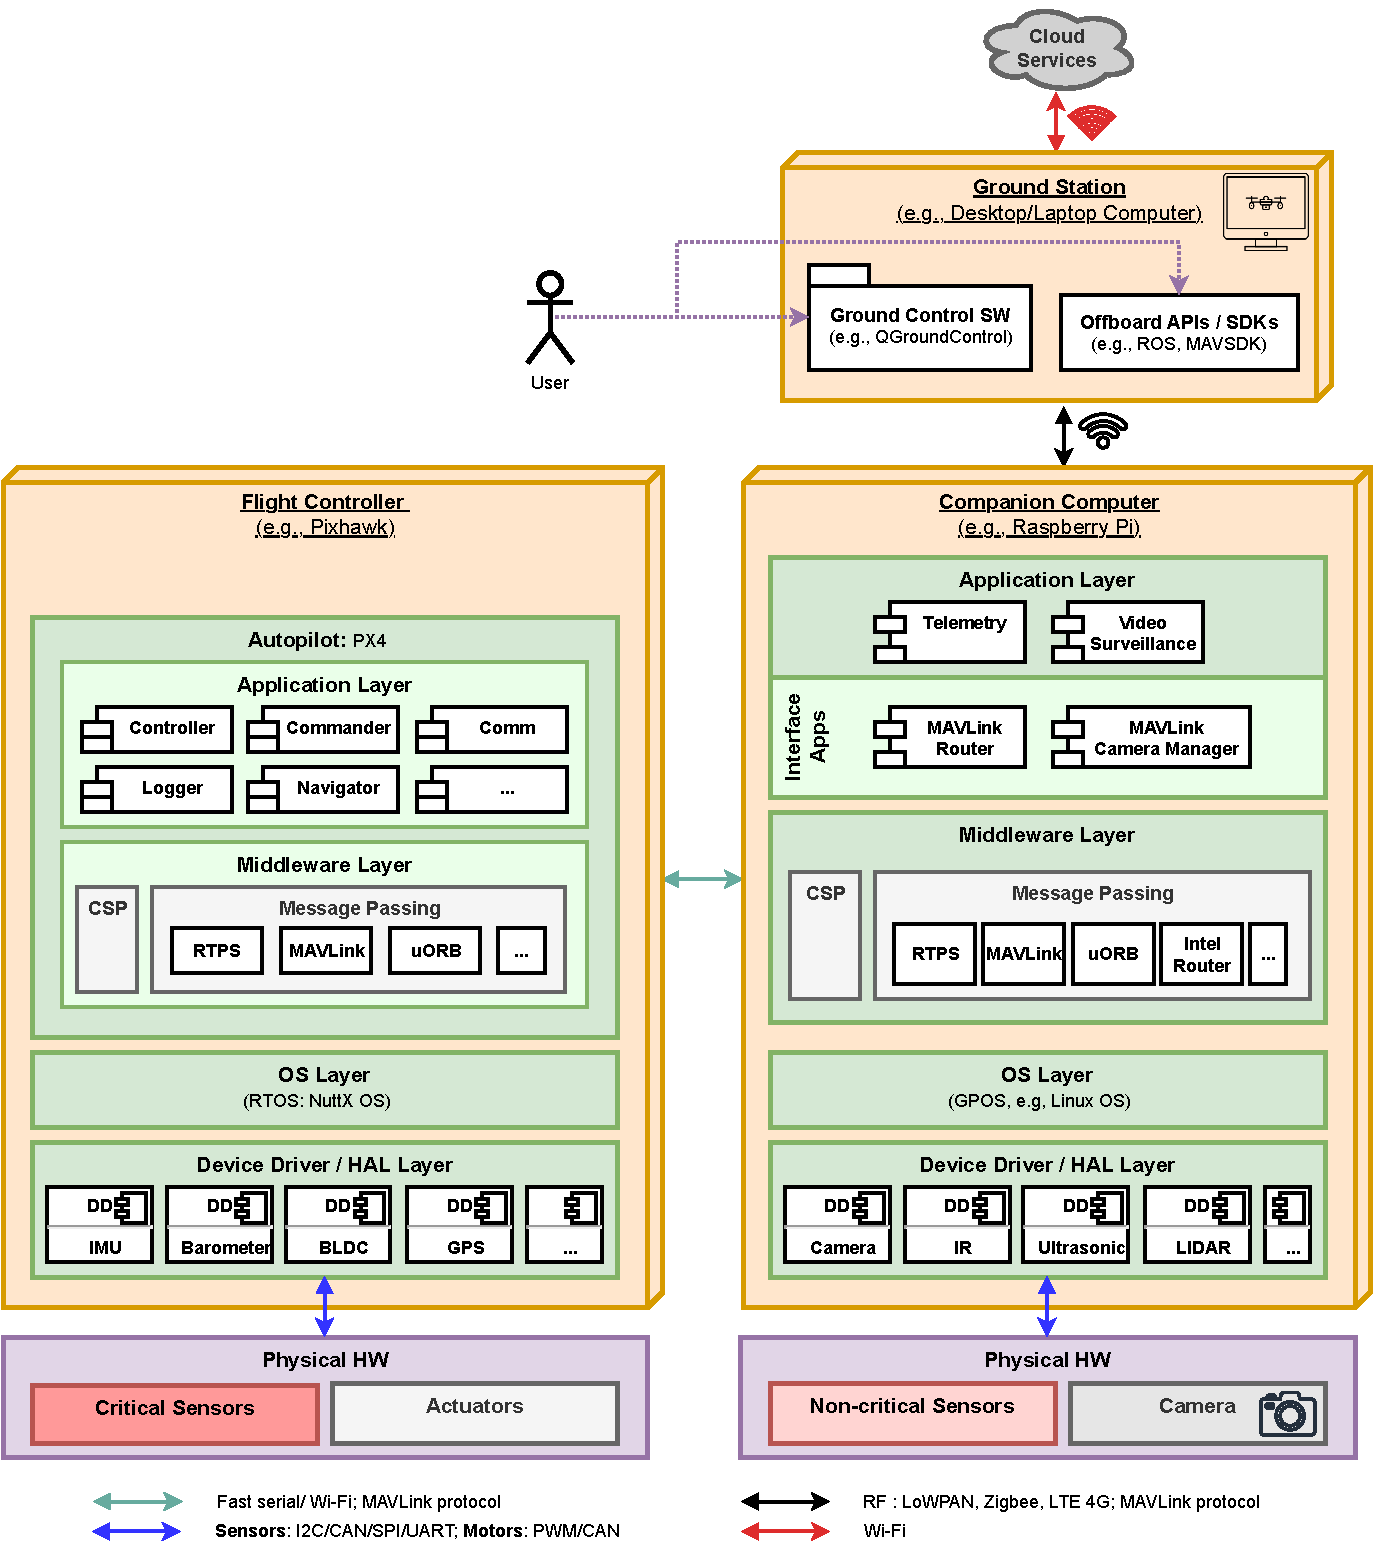
\includegraphics[width=0.9\textwidth]{./img/pdf/uav-main-design-conv-sol-1.pdf}
  \caption{UAV design: conventional solution (full).}
  \label{fig:uav-design-conv-sol-1}
\end{figure}

We adopt the PX4 flight stack for its open model, broad platform support,
modular architecture, and industrial adoption. PX4 runs on the flight controller
atop NuttX. In a typical setup, the Companion Computer routes communication
between the \gls{gcs} and the \gls{fmu}: a fast serial or Ethernet link
(\gls{uart} or Ethernet) is established between the \gls{fmu} and the Companion
Computer using MAVLink; the Companion Computer runs auxiliary routing software
(e.g., MAVLink Router~\cite{px4-routers}). The \lstinline|User| interacts with
\emph{QGroundControl} for configuration and supervision and may also use
offboard \glspl{api}/\glspl{sdk} (e.g., \lstinline|MAVSDK|) to interact with the
Companion Computer. The \gls{rc} link is omitted here because manual flight is
not central to the video-surveillance use case.

Camera control usually requires an additional service on the Companion Computer,
such as the MAVLink Camera Manager~\cite{px4-cam-managers}, which bridges PX4’s
MAVLink Camera Protocol v2 to the camera’s native protocol. This indirection
adds complexity and latency. More importantly, it increases risk: if the
Companion Computer is compromised, the \gls{fmu} can be affected via corrupted
data or link disruption.

Figure~\ref{fig:uav-design-conv-sol-2} presents a simplified conventional
variant specialized for video surveillance, with tighter decoupling between
telemetry and payload video.
%
Dedicated links are used for \gls{gcs}\,$\leftrightarrow$\,\gls{fmu} telemetry
(e.g., radio) and for camera streaming (e.g., Wi-Fi). To simplify networking and
avoid extra hardware, the \gls{gcs} and the \gls{uav} share the same \gls{lan}.
The video subsystem is split into a client on the \gls{gcs} and a server on the
Companion Computer, each exposing a control port (e.g., 5000). The client sends
commands to the server, which configures a capture/encode pipeline and streams
frames back; the receiver on the \gls{gcs} sets up a matching pipeline for
decode and display. Occasional frame loss is acceptable for situational
awareness, so a connectionless transport such as \gls{udp} is appropriate
(lower overhead and reduced blocking compared with reliable
streams). This simplified conventional design serves as the baseline for our
subsequent platform unification.

\begin{figure}[!hbt]
  \centering
  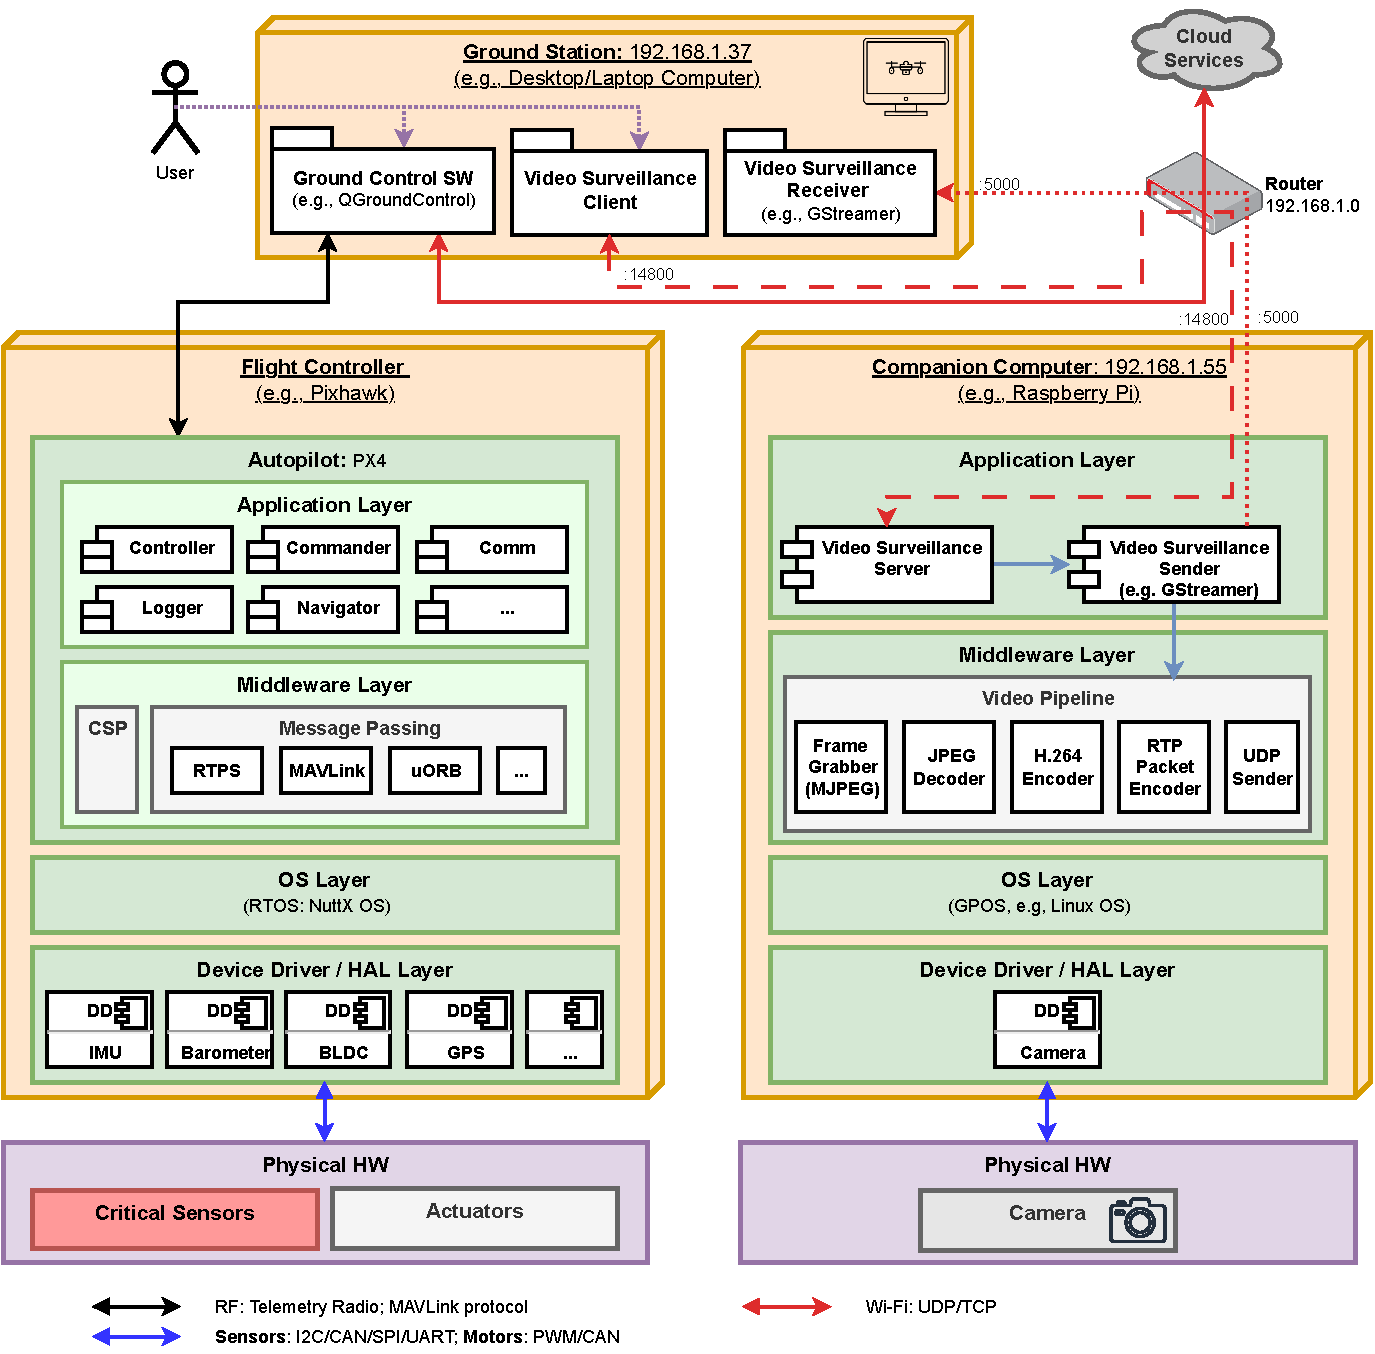
\includegraphics[width=0.9\textwidth]{./img/pdf/uav-main-design-conv-sol-2.pdf}
  \caption{UAV design: conventional solution (simplified).}
  \label{fig:uav-design-conv-sol-2}
\end{figure}


\subsection{Unsupervised Single-Platform Flight Stack}
\label{sec:unsuperv-stack}

Integrating the \gls{fmu} and the companion-computer functionality on a single
platform requires encapsulating both as standalone components. In the
\glsxtrfull{uspfs}, these components are realized as processes on a \gls{gpos}.

Figure~\ref{fig:uav-design-unsup} shows the \gls{uspfs} architecture. Software
processes for the \gls{gcs} and the \gls{uavic} are shown in blue. The
\gls{uavic} consolidates \gls{fmu} and companion roles on one Linux platform:
PX4 runs on core~0, while the remaining cores are allocated to the video
surveillance application.

\begin{figure}[!hbt]
  \centering
  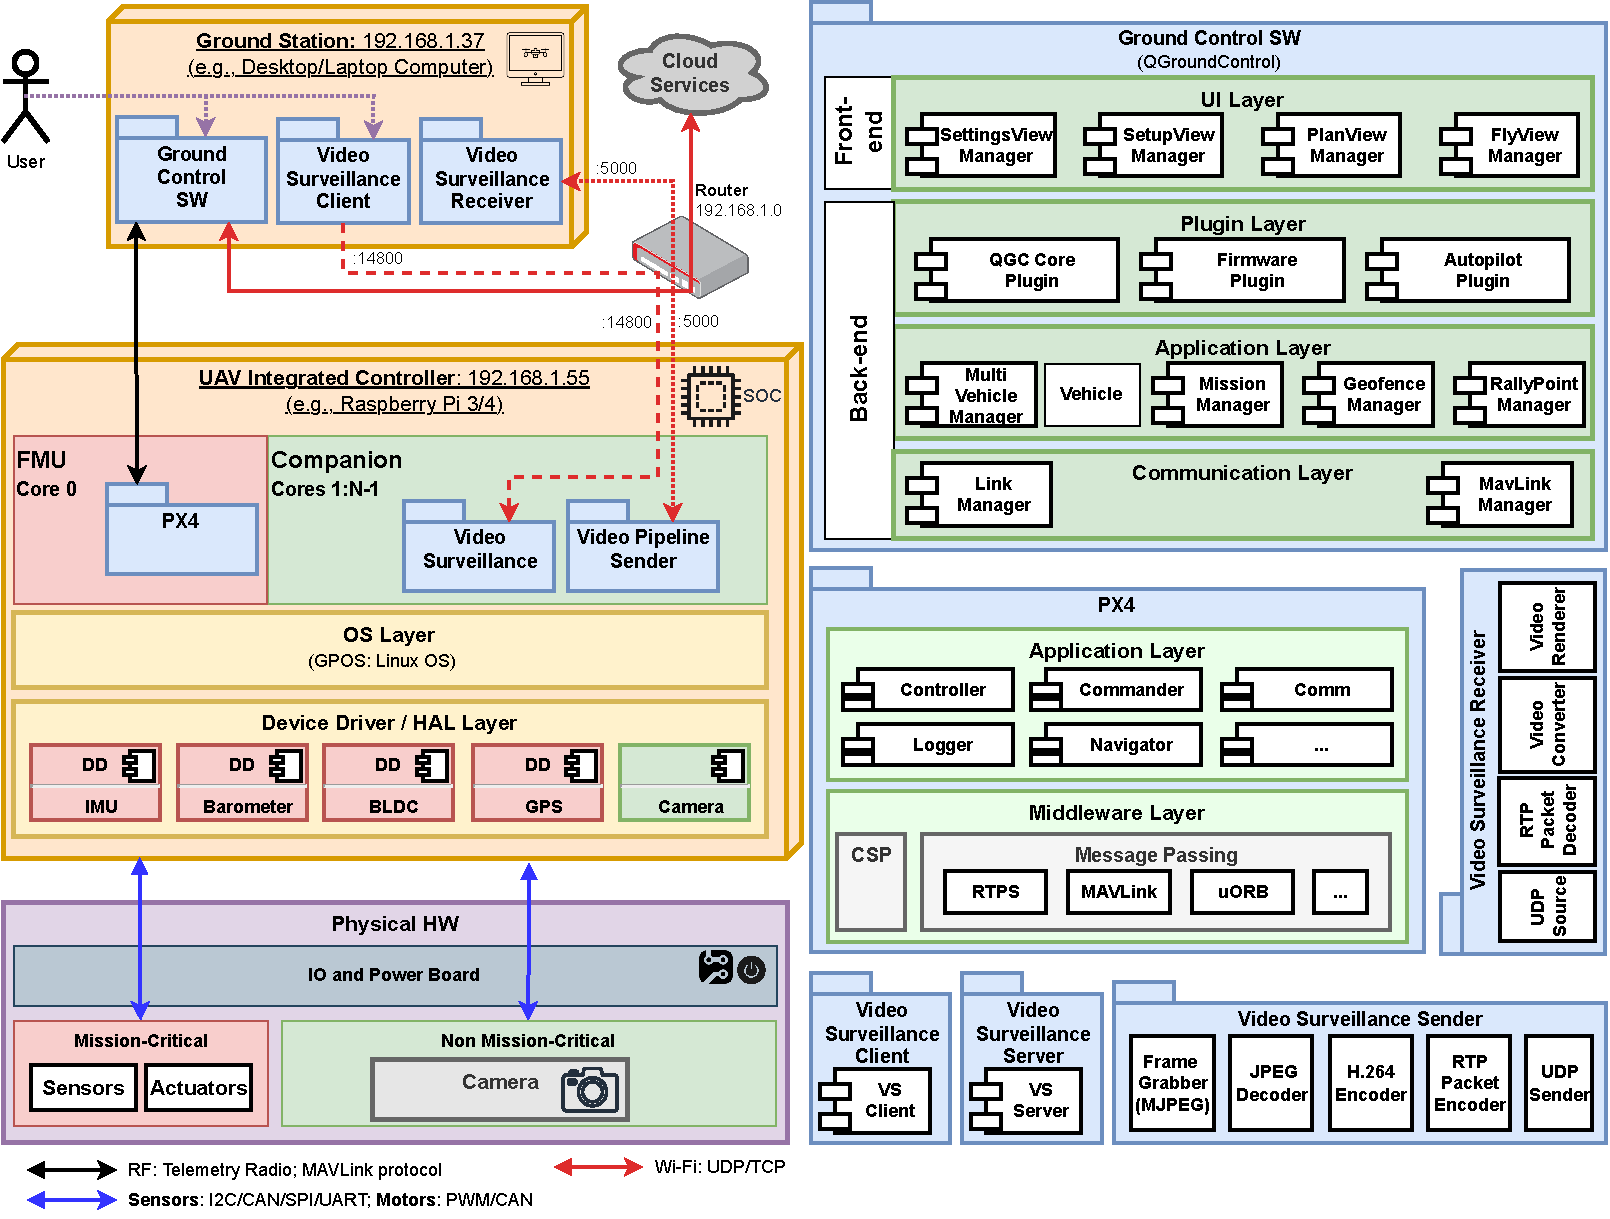
\includegraphics[width=1.0\textwidth]{./img/pdf/uav-main-design-unsup.pdf}
  \caption{UAV design: unsupervised single-platform flight stack.}
  \label{fig:uav-design-unsup}
\end{figure}

Because PX4 no longer runs on NuttX, meeting soft real-time requirements becomes
more challenging. To mitigate this on Linux, we (i) dedicate a CPU to PX4, (ii)
use a real-time kernel configuration (e.g., \texttt{PREEMPT\_RT}) with suitable
\gls{io} scheduling, and (iii) set IRQ and thread affinities with
priority policies appropriate for the control loop.

Despite these mitigations, this architecture provides no strong isolation: faults
or overloads in non-critical processes can impact the PX4 process and its
resources. This propagation risk makes the unsupervised design insufficient as a
final solution; supervision is required to ensure reliable consolidation and
safe integration.

\subsection{Supervised Single-Platform Flight Stack}
\label{sec:superv-stack}

Figure~\ref{fig:uav-design-sup} shows the \glsxtrfull{sspfs}. The \gls{fmu} and
companion roles are realized as guest \glspl{vm} running atop the Bao
hypervisor on the \gls{uavic}. This design provides strong isolation between
mixed-criticality domains so that faults in the non-critical stack do not impact
the \gls{fmu}.

\begin{figure}[!hbt]
  \centering
  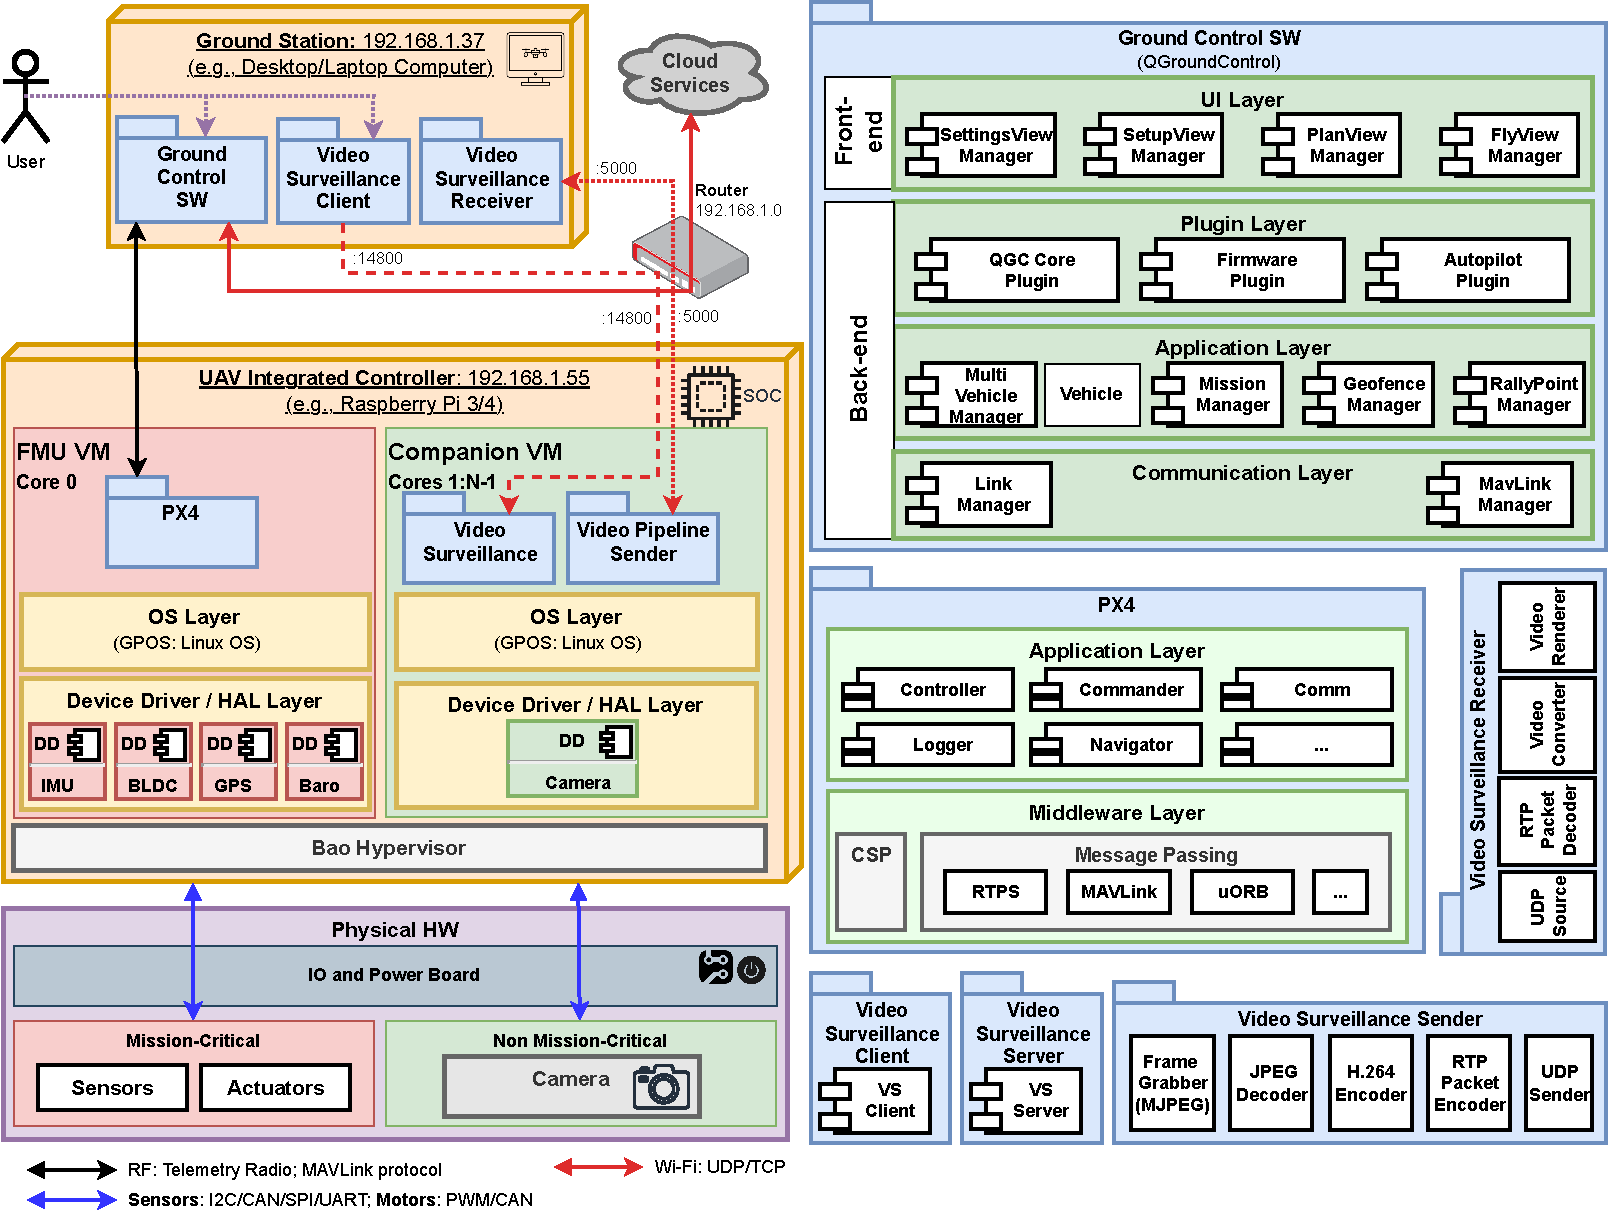
\includegraphics[width=1.0\textwidth]{./img/pdf/uav-main-design-sup.pdf}
  \caption{UAV design: supervised single-platform flight stack.}
  \label{fig:uav-design-sup}
\end{figure}

Each \gls{vm} runs a Linux-based \gls{os}, enabling tailored configurations. The
\gls{fmu} \gls{vm} can use a real-time kernel and be pinned to a dedicated CPU,
while the companion \gls{vm} can run a standard kernel. Bao’s static
partitioning assigns CPUs, memory, and devices to each \gls{vm} exclusively,
and device drivers reside within the respective guest, limiting the effects
of software bugs.

The main costs are footprint and configuration effort: every \gls{vm} carries a
full \gls{os}, increasing binary size and memory use, and the \lstinline|User|
must select and assign hardware resources carefully to avoid contention while
meeting performance targets for \gls{cpu}, memory, and I/O. In practice, the
mapping may need small adjustments to the chosen hardware platform.

\section{Hardware Selection}
\label{sec:hardware-selection}
This section selects hardware for the \gls{uav}, the \gls{uavic}, and required
add-ons. Choices are mapped to PX4 requirements and to constraints imposed by
Bao on the \gls{uavic}.

\subsection{UAV}
\label{sec:uav-hw-sel}
We target a multirotor airframe due to its availability, compact form factor,
and \gls{vtol} capability that reduces takeoff area. Operations are assumed at
low altitude for regulatory and operational reasons. We also favor a high
power-to-weight ratio to extend flight endurance.
%
Figure~\ref{fig:hoverGames-drone} shows the selected platform:
\lstinline{KIT-HGDRONEK66}, commonly known as the NXP HoverGames \gls{uav}
kit~\cite{nxp-hoverGames-uav}. This professional DIY kit, priced under
USD~500, includes the RDDRONE-FMUK66 as the \gls{fmu} \emph{(1)}.

\begin{figure}[!hbt]
  \centering
  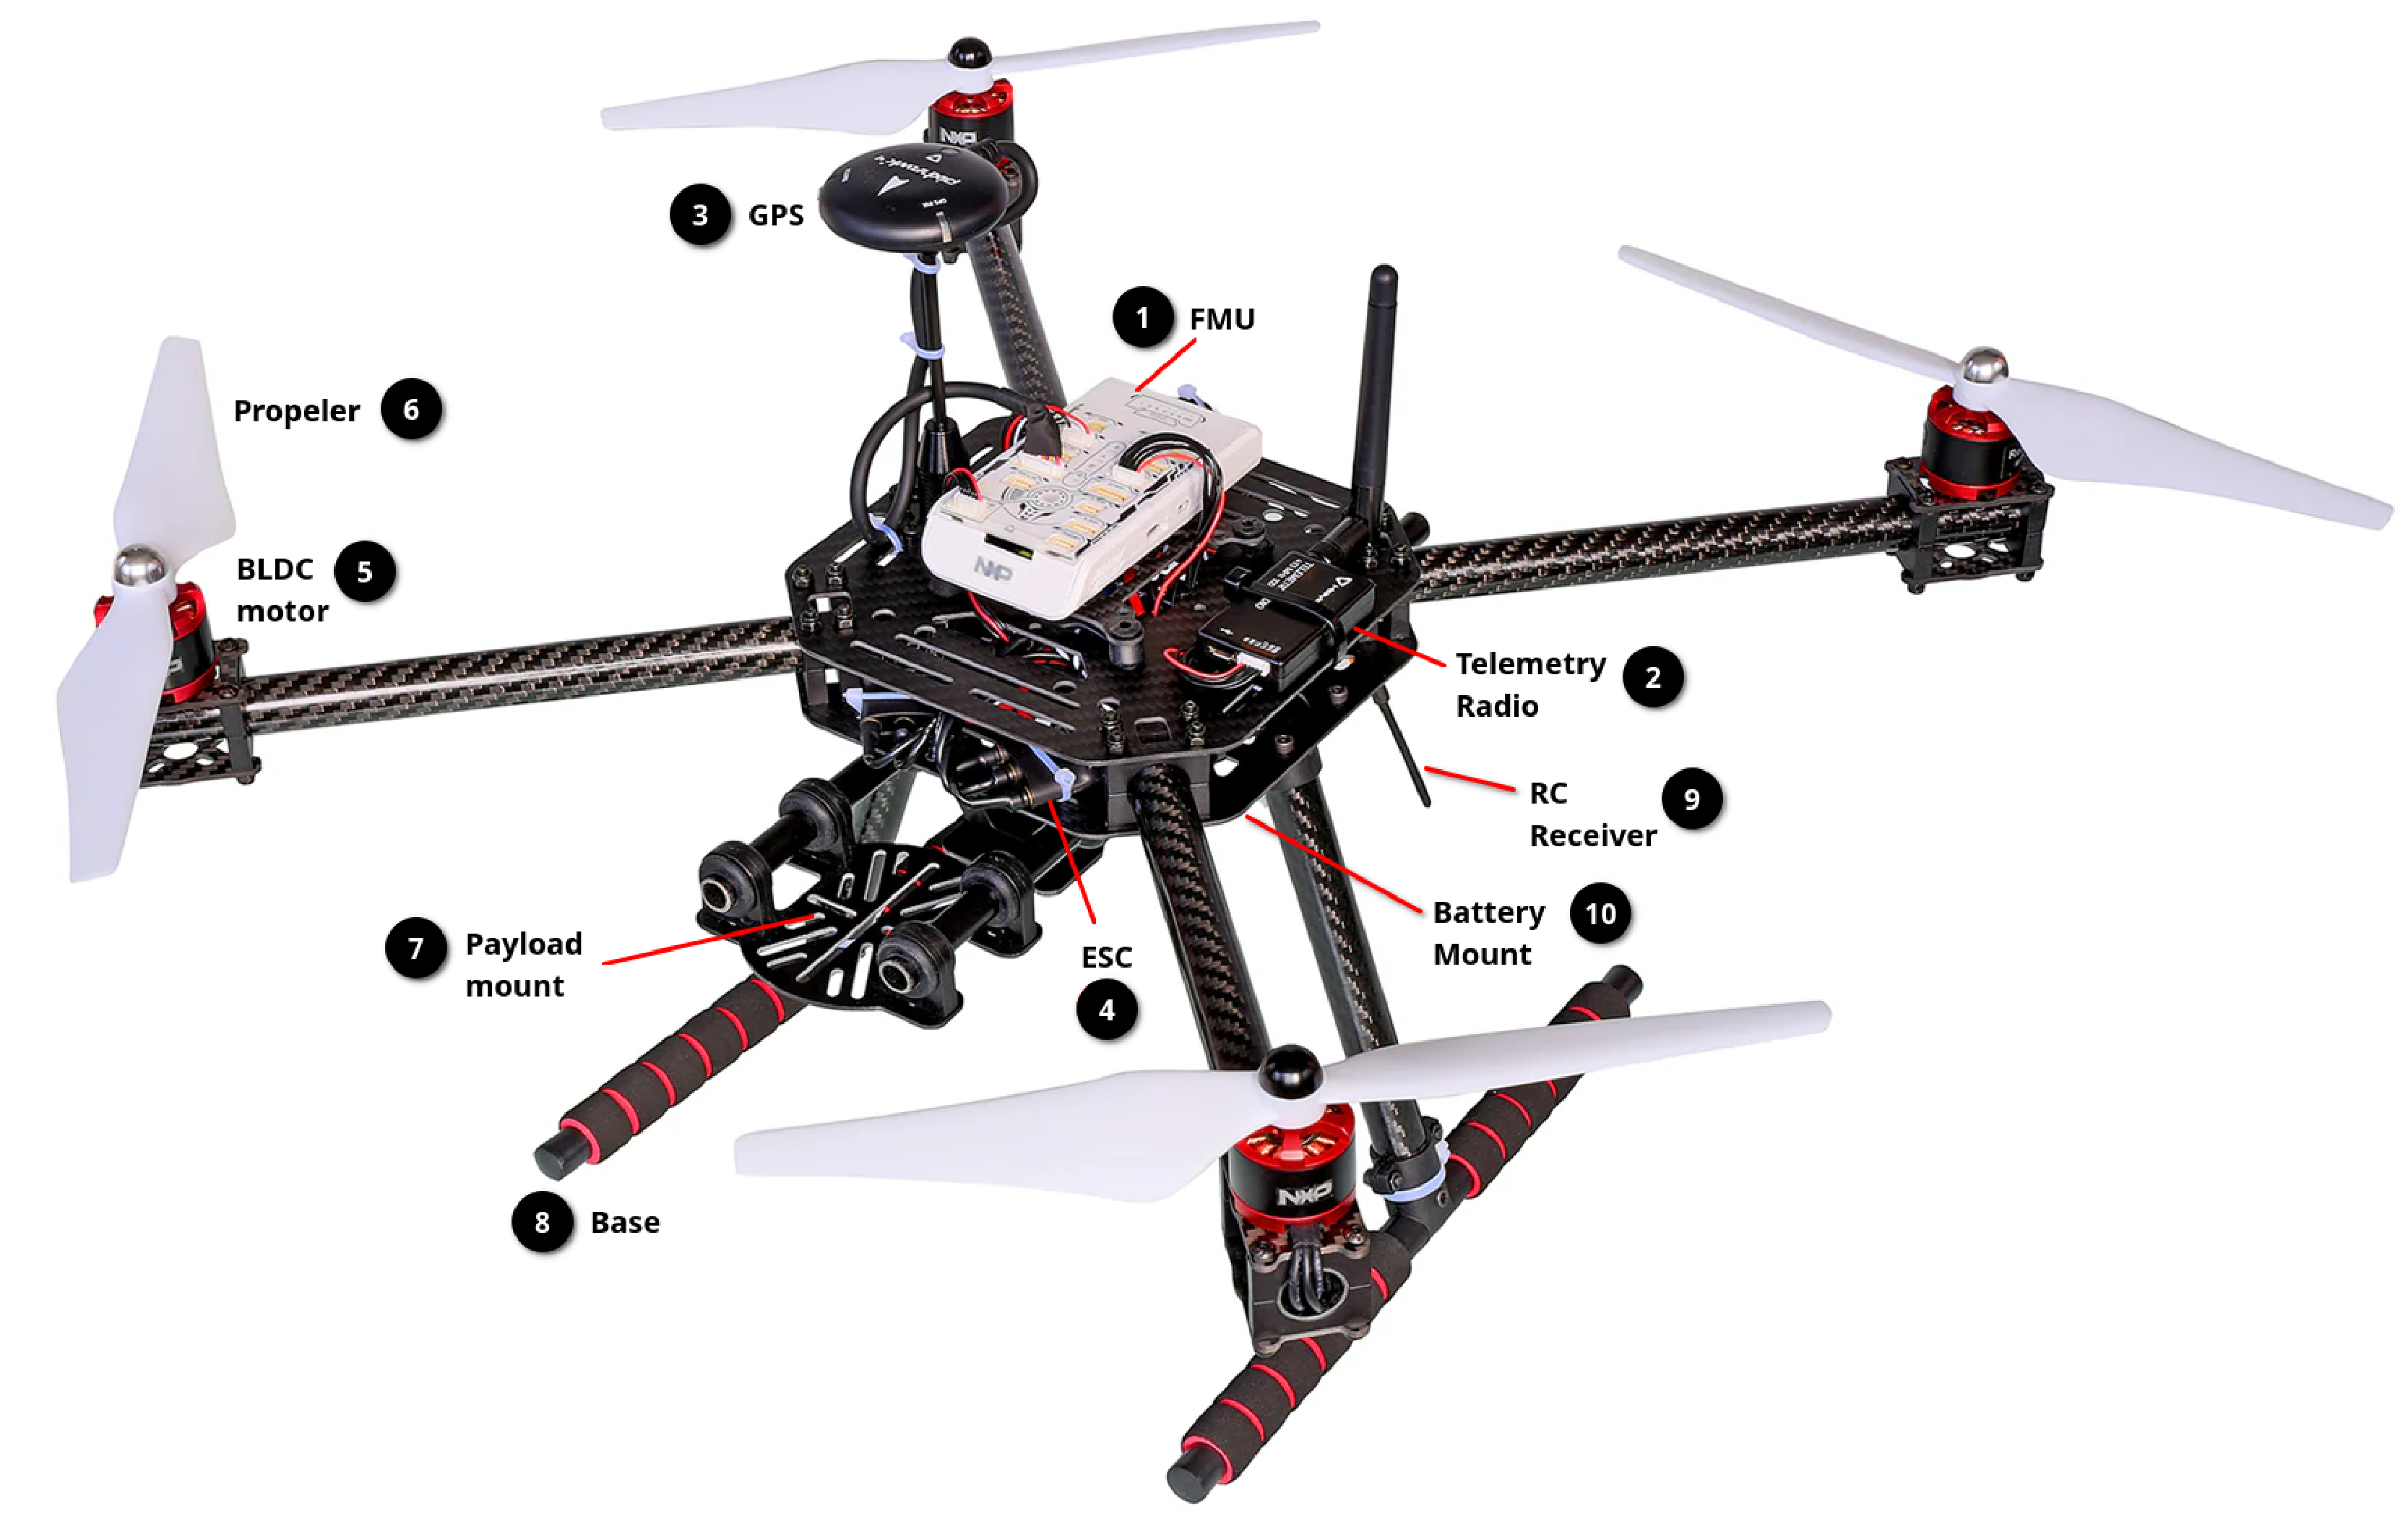
\includegraphics[width=1.0\textwidth]{./img/pdf/hoverGames-drone.pdf}
  \caption[NXP HoverGames UAV kit]{NXP HoverGames UAV kit (adapted from~\cite{nxp-hoverGames-uav})\footnotemark}
  \label{fig:hoverGames-drone}
\end{figure}
\fnlicNC{NXP Semiconductors}

The kit uses an S500 carbon-fiber quadcopter frame (500\,mm wheelbase) with
\gls{bldc} motors \emph{(5)} driving the propellers \emph{(4)}, each controlled by an
\gls{esc} \emph{(6)}. For autonomous flight it includes a \gls{gps} module \emph{(3)}
and a payload mount \emph{(7)} for accessories such as cameras. Power is supplied by a
3S \gls{lipo} battery (purchased separately) in the 3500–5000\,mAh range. A
telemetry radio \emph{(2)} (purchased separately) can be connected to the \gls{fmu};
in Europe a 433\,MHz variant is typically used. The kit also includes an
\gls{rc} transmitter (GS-i6S) and a receiver.

Figure~\ref{fig:hoverGames-blkDiag} depicts the block diagram. The
RDDRONE-FMUK66 \gls{fmu} integrates an NXP Kinetis\textsuperscript{\textregistered} K66
\gls{mcu} (Arm\textsuperscript{\textregistered} Cortex\textsuperscript{\textregistered}-M4 at 180\,MHz,
2\,MB flash, 256\,KB \gls{sram})~\cite{nxp-hoverGames-fmu} running the PX4
autopilot. A power-distribution board provides current and voltage sensing for
battery-state estimation. The \gls{fmu} interfaces typical sensors
(accelerometer, gyroscope, magnetometer, barometer) and actuators
(\gls{bldc} via \gls{pwm}, servos where applicable). Communication with a
companion computer is via \gls{uart}; links to the \gls{gcs} are provided by a
telemetry radio or an \gls{rc} link. An optional \gls{sd} card enables flight
logging for offline analysis and simulation replay. A SEGGER J-Link EDU Mini
\gls{swd} adapter supports on-target debugging and firmware upload to the \gls{fmu}.

\begin{figure}[!hbt]
  \centering
  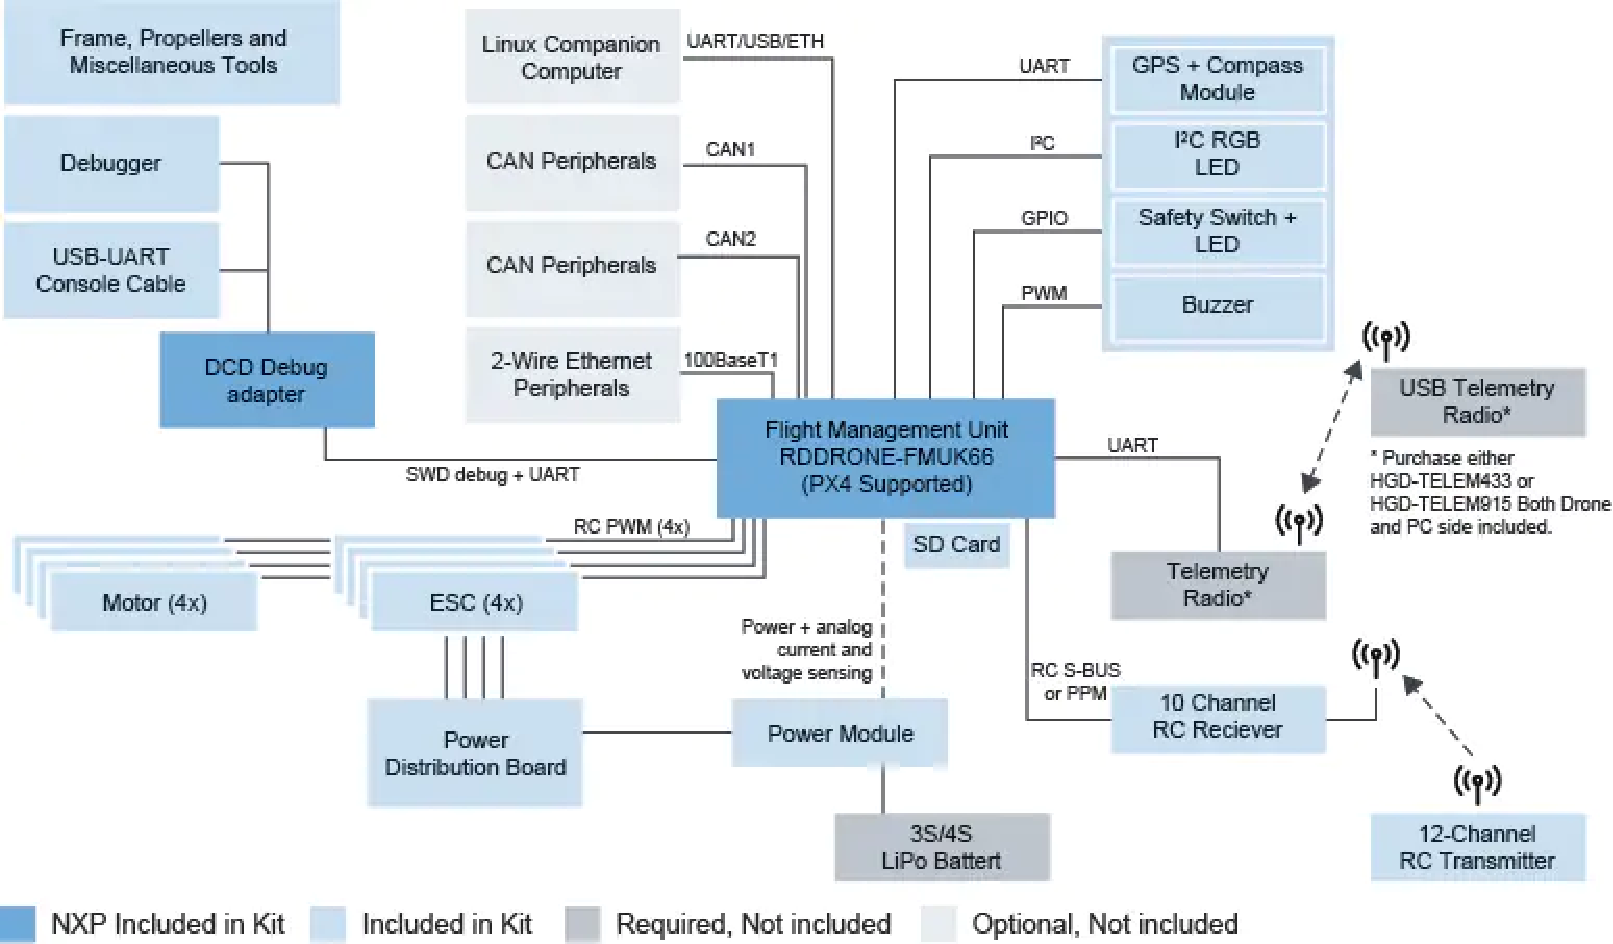
\includegraphics[width=1.0\textwidth]{./img/pdf/hoverGames-blkDiag.pdf}
  \caption[NXP HoverGames block diagram]{NXP HoverGames block diagram (adapted from~\cite{nxp-hoverGames-uav})\footnotemark}
  \label{fig:hoverGames-blkDiag}
\end{figure}
\fnlicNC{NXP Semiconductors}


\subsection{UAV Integrated Controller}
\label{sec:uav-integr-contr}
The \glsxtrfull{uavic} merges \gls{fmu} and companion-computer functionality on
a single platform. For mixed criticality, the ideal design separates computing
domains, e.g., a real-time processor for the \gls{fmu} and a general-purpose
processor for the companion stack. This points to a heterogeneous \gls{soc},
such as the NXP i.MX~8M Nano~\cite{imx8mn}, which integrates an Arm\textsuperscript{\textregistered}
Cortex\textsuperscript{\textregistered}-M7 (well suited to NuttX) and a quad-core
Cortex\textsuperscript{\textregistered}-A53 (well suited to a Linux \gls{os}). However, the NuttX \gls{rtos}
does not currently support this board~\cite{nuttx-platforms}.

Our initial plan was to port NuttX to the Cortex-M7 and then enable PX4 on that
target, including the required device drivers. In parallel, Bao support for this
board would be needed also. The combined effort (new NuttX port, PX4 enablement,
and Bao enablement) proved impractical for this work’s scope, so we adopted a
more direct path.
%
We next considered running PX4 directly on Linux with a real-time kernel and
appropriate \gls{io} scheduling to limit latency. PX4’s Linux support, however,
is restricted to a small set of platforms (e.g., BeagleBone Blue and
Raspberry~Pi~2/3/4 with specific shields)~\cite{px4-experimental-autopilot},
which constrained options. Consequently, we consolidated each software stack
into its own Linux \gls{os} \gls{vm}, rather than splitting across heterogeneous cores.

As the host platform, we selected Raspberry~Pi~4 paired with the PilotPi shield,
balancing availability, documentation quality, and cost. Fig.~\ref{fig:pilotpi-annot}
shows the resulting \gls{uavic}. The Raspberry Pi 4 Model B (1) runs a Linux-based
\gls{os} from the \gls{sd} card and exposes \gls{csi} camera and \gls{usb}
interfaces. It features the Broadcom BCM2711 \gls{soc} with a 64-bit quad-core
Arm\textsuperscript{\textregistered} Cortex\textsuperscript{\textregistered}-A72 at 1.8\,GHz and a
VideoCore~VI \gls{gpu} at 500\,MHz~\cite{rpi4-specs,rpi4-bcm2711}, plus 8\,GB
LPDDR4-3200 SDRAM. Connectivity includes dual-band 802.11ac, Bluetooth~5.0,
Gigabit Ethernet, two \gls{usb}~3.0 ports, and two \gls{usb}~2.0 ports.

The sensor board (2) mounts atop the Raspberry Pi, providing \gls{gps}, telemetry,
and \gls{rc} external interfaces mapped to \lstinline{/dev/ttySC0}, \lstinline{/dev/ttySC1},
and \lstinline{/dev/ttyAMA0}, respectively. Onboard sensors include an accelerometer/gyroscope
(\lstinline{ICM42688P}), a magnetometer (\lstinline{IST8310}), and a barometer
(\lstinline{MS5611}) required by PX4.
%
The topmost layer contains the power board (3), which handles power supply (8),
monitoring (11), and motor actuation via \gls{pwm} (10) using the Linux
\lstinline{PCA9685} driver. A header exposes unused pins, enabling additional
connections such as a remote serial interface (UART5).

\begin{figure}[!hbt]
  \centering
  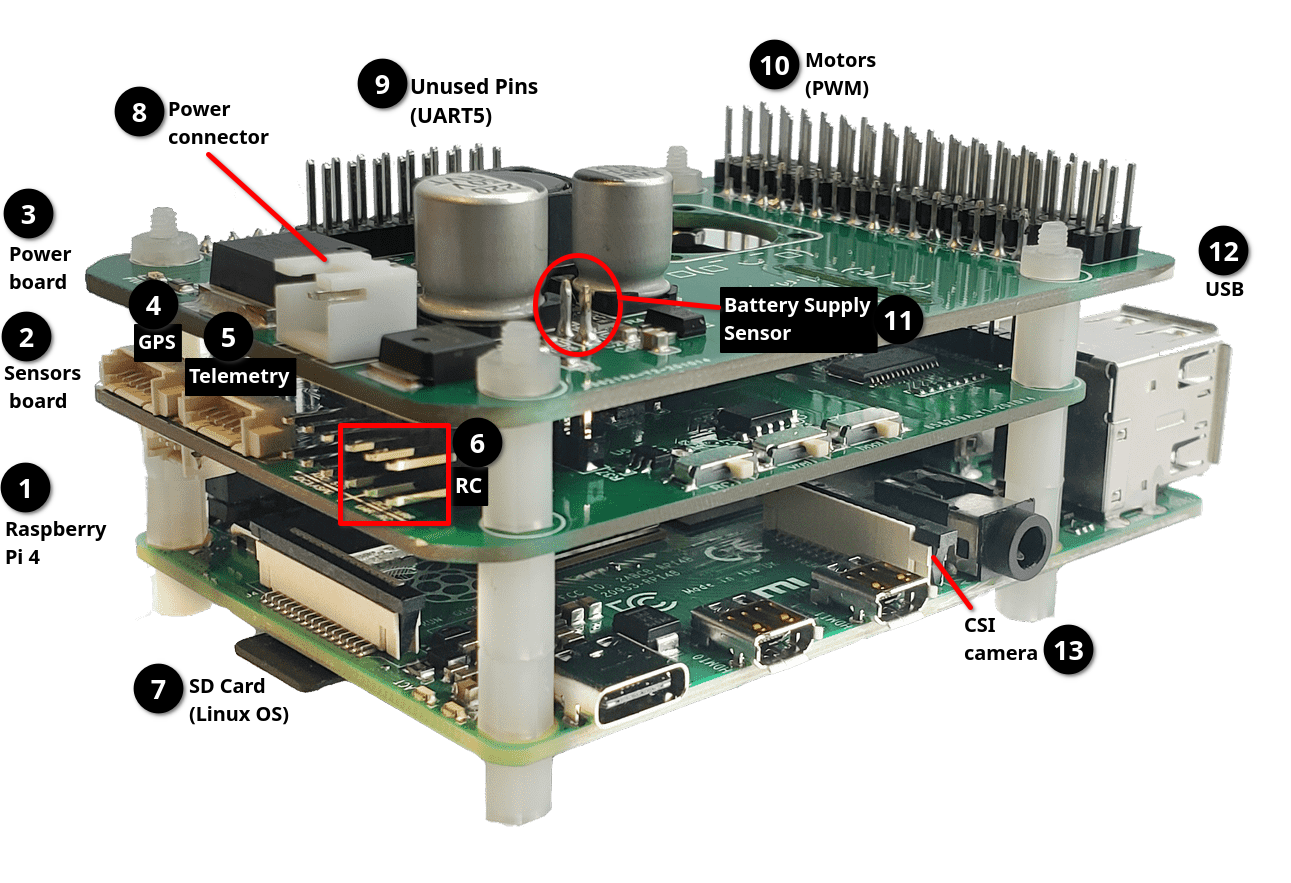
\includegraphics[width=0.9\textwidth]{./img/png/pilotpi-annotated}
  \caption[UAVIC: Raspberry Pi 4 + PilotPi shield]{UAVIC: Raspberry Pi 4 +
    PilotPi shield (adapted from~\cite{px4-pilotpi})\footnotemark}
  \label{fig:pilotpi-annot}
\end{figure}
\fnlicCCFour{foot:pilotpi-annotated}%

\subsection{Hardware mapping}
\label{sec:hardware-mapping}
The \gls{uavic} platform must satisfy PX4 requirements for sensors and
actuators. Because the Bao hypervisor enforces static partitioning, we must also
determine whether the \gls{uavic} hardware can be made fully available to each
guest in the \gls{sspfs} solution or if alternatives are needed.
Accordingly, we first map the PX4-required hardware to the Linux device tree for
the \gls{uspfs} solution and then adapt that mapping to meet Bao's constraints
in the \gls{sspfs} implementation.

\subsubsection{USPFS}
\label{sec:base-scenario}
Fig.~\ref{fig:hw-map-1} depicts the full device tree for the \gls{uavic} system,
representing the \gls{uspfs} solution (base scenario).
Solid lines denote aggregation (e.g., the \lstinline{root} node includes the \lstinline{memory} node);
dashed lines denote dependency (e.g., the \lstinline{power} and \lstinline{firmware} nodes depend on \lstinline{mailbox}).
%
The coloring highlights functional groupings:
\begin{itemize}
  \item \hlighthex{ADD8E6}{000000}{Generic nodes}: essential for all Raspberry~Pi~4 configurations
    (e.g., \lstinline{memory}, \lstinline{cpus}, \lstinline{power-regulator}).
  \item \hlighthex{FFE4C4}{000000}{PX4-required nodes}: \lstinline{i2c1} (motor actuation),
    \lstinline{spi0} (\gls{imu}, barometer, magnetometer), \lstinline{spi1} (\gls{gps}, telemetry radio),
    and \glspl{uart}~0/5 (\gls{rc} link, debug console).
  \item \hlighthex{90EE90}{000000}{Companion VM nodes}: \lstinline{i2c0} and \lstinline{csi1} (camera),
    \lstinline{mmcnr} (Wi-Fi support).
  \item \hlighthex{FFB6C1}{000000}{Firmware nodes}: enable \gls{gpu}–\gls{cpu} communication via \lstinline{mailbox}~\cite{rpi4-fw-mbox}.
\end{itemize}

\begin{figure}[!hbt]
  \centering
  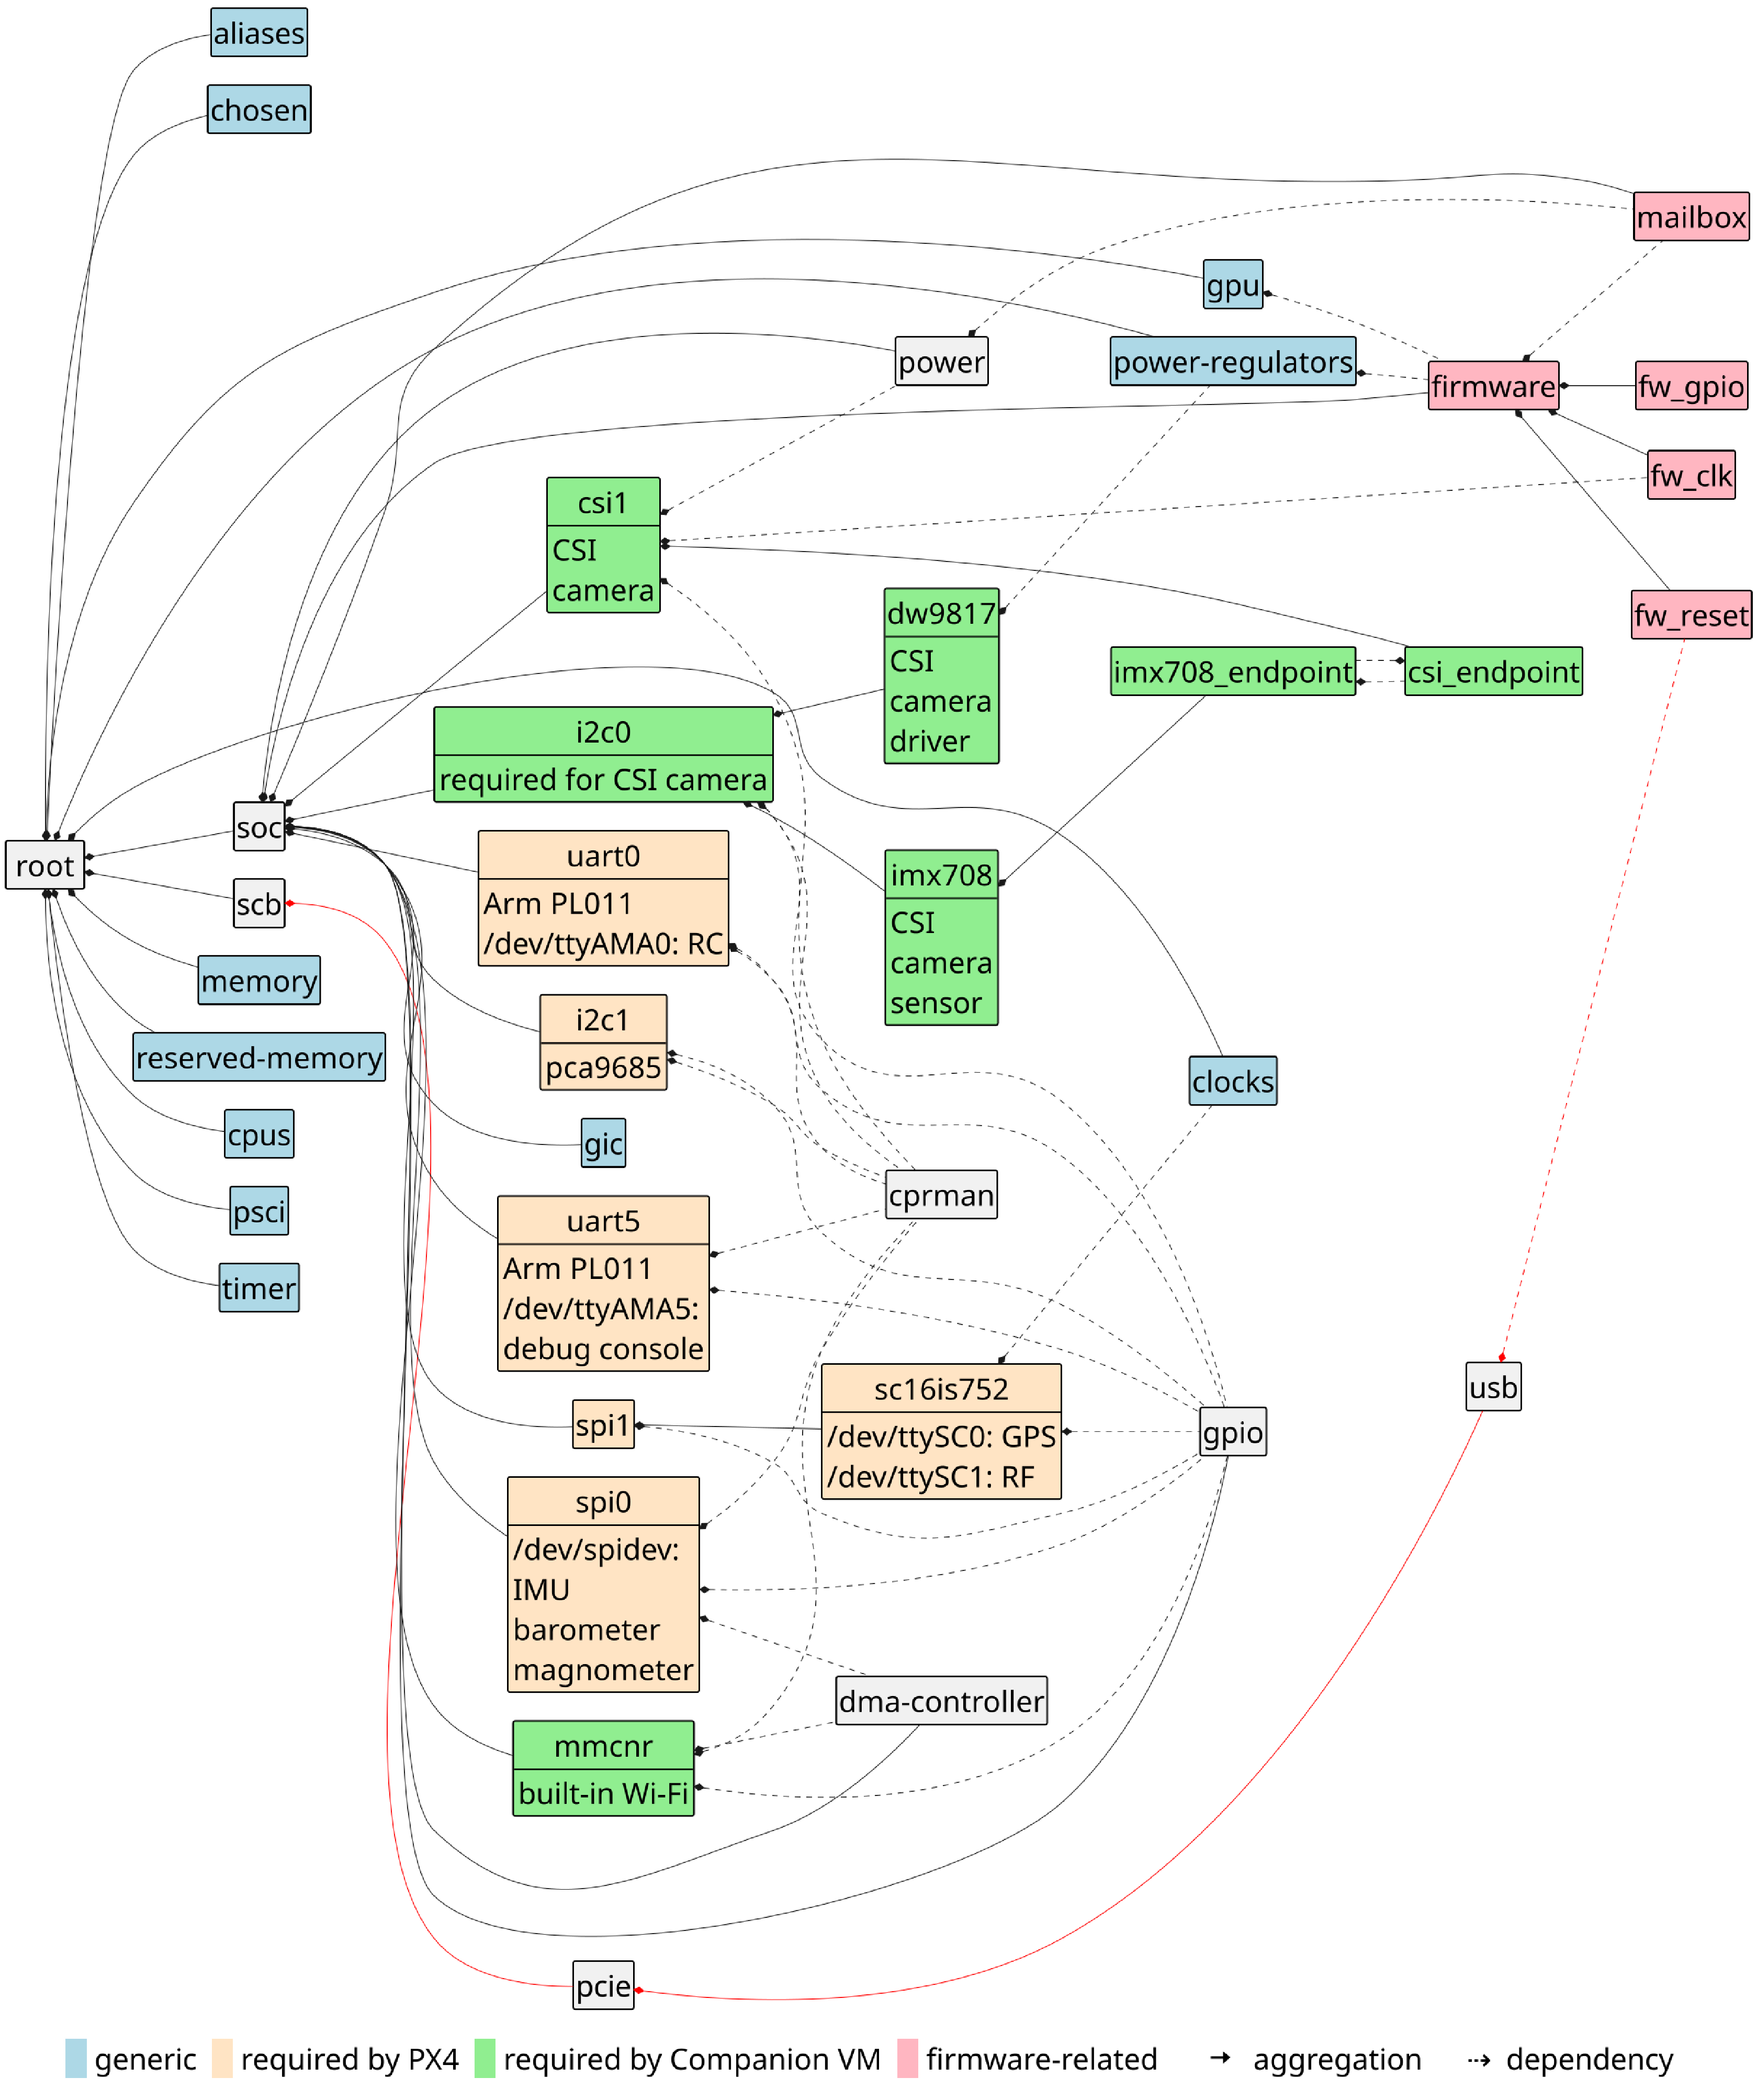
\includegraphics[width=0.85\textwidth]{./img/pdf/hw-map-1}
  \caption[Hardware mapping: USPFS device tree]{Hardware mapping: \gls{uspfs} device tree}
  \label{fig:hw-map-1}
\end{figure}

Device-tree analysis reveals several shared dependencies between PX4 and the
Companion \gls{vm}: the clock manager (\lstinline{cprman}), the \gls{gpio}
controller, and the \gls{dma} controller. Because Bao’s isolation model
prohibits device sharing, an alternative architecture is required.

We retain PX4's native device set and migrate Companion \gls{vm} devices to the
\gls{usb} interface. As indicated by the dependency path (red line), the
\lstinline{usb} device (under \lstinline{pcie}) shares only the
\lstinline{firmware} node with PX4, which itself depends on \lstinline{mailbox}.
This simplifies the \gls{sspfs} design, but shared \lstinline{mailbox} access
must be reconciled with Bao. Removing \lstinline{firmware} from either \gls{vm}
would break the system, so this is infeasible.
%
Accordingly, we combine the Companion \gls{vm} migration to \gls{usb} with
supervised mailbox access in Bao. This preserves hardware isolation while
enabling secure use of the required shared resource.

\subsubsection{Supervised mailbox access}
\label{sec:superv-mailb-access}
Fig.~\ref{fig:design-mailbox} illustrates the mailbox access for the
conventional case (left) and the supervised one (right).
%
The solid lines denote synchronous events, while the dashed lines denote
asynchronous ones.
\textcolor{red}{Red} arrows indicate the outgoing path (from the mailbox
driver), and \textcolor{blue}{blue} arrows indicate the incoming path. Mailbox
transactions are shown as white (conventional), violet (VM1), and grey (VM2)
envelopes. The synchronization mechanisms (locks) appear in brown for the
mailbox and in blue for Bao. Hypercalls are shown as phones: green for
\lstinline{Start_TX} and red for \lstinline{End_TX}. Numbered labels mark the
event sequence in each case.

\begin{figure}[!hbtp]
  \centering
  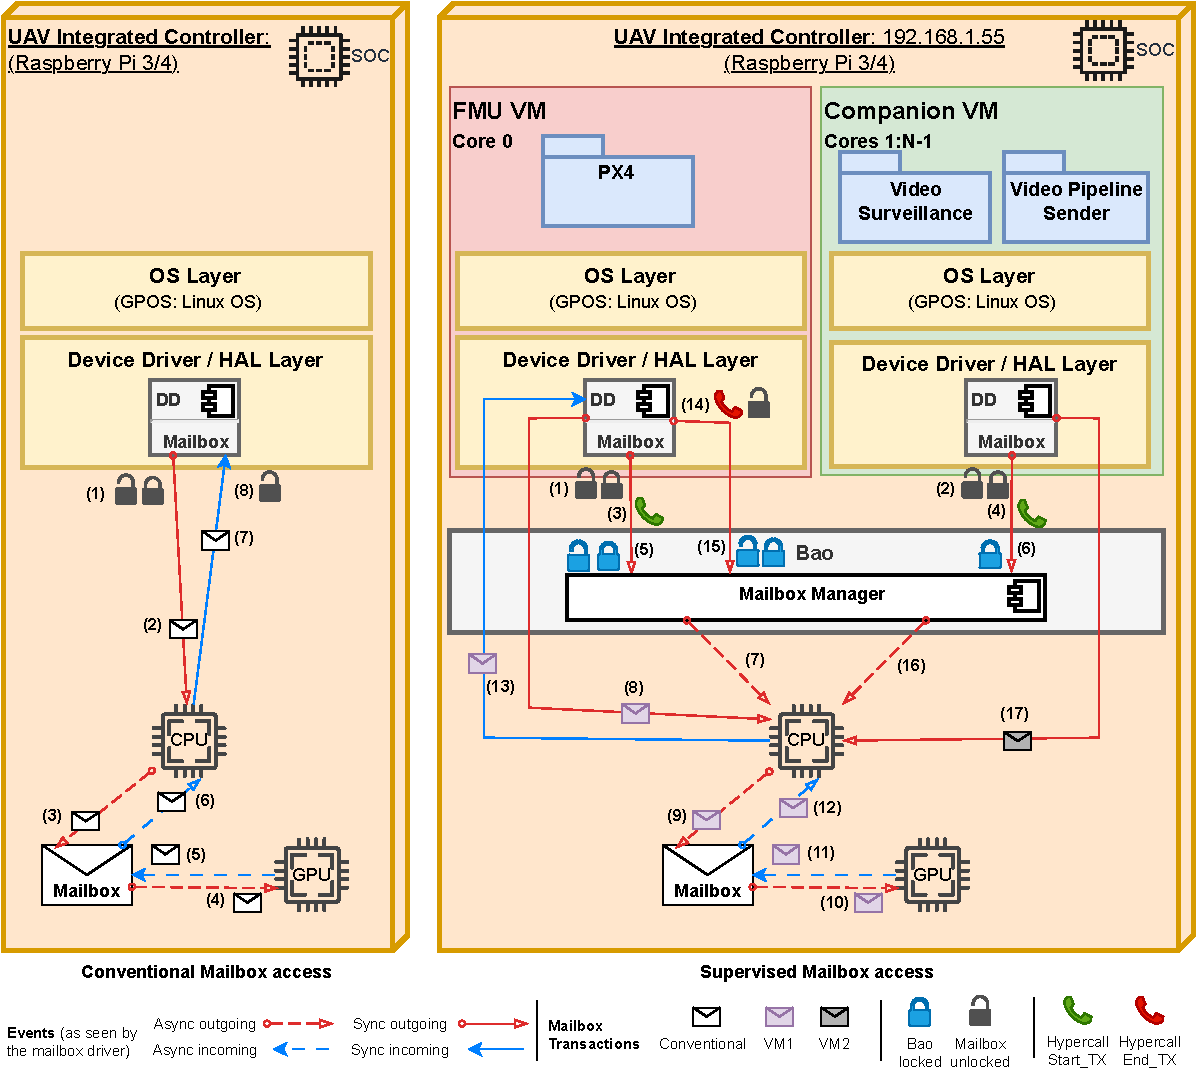
\includegraphics[width=1.0\textwidth]{./img/pdf/uav-main-design-mailbox}
  \caption{Mailbox access: conventional (left); supervised (right)}%
  \label{fig:design-mailbox}
\end{figure}


In the conventional case, the mailbox device driver can initiate a transaction
request if no other is pending \emph{(1)}. The transaction must
be completed \emph{(8)} before a timeout occurs, freeing the mailbox for further
requests. An interrupt is triggered \emph{(2)} and the \gls{cpu} forwards the request
to the mailbox \emph{(3)} which requests data from the \gls{gpu} \emph{(4)}. The \gls{gpu}
firmware handles the transaction and returns a result to the mailbox \emph{(5)}. The
mailbox forwards the response to the mailbox's driver \emph{(6), (7)}, completing
the request and freeing the mailbox~\cite{rpi4-mbox-driver}.

In the supervised case, VM1's mailbox driver attempts to start a
transaction when none is pending \emph{(1)}. Now,
before transmission, the mailbox driver must signal to Bao it wants
to start a transaction by performing a \lstinline{Start_TX} hypercall \emph{(3)}. Bao
acknowledges this request if no transaction is ongoing, locking the
mailbox manager \emph{(5)}.
VM2 performs the same attempt \emph{(2), (4)} but must wait because VM1 holds the lock.
%
The mailbox manager handles the hypercall,
associates the guest, target device (mailbox), and interrupt ID, and injects the
interrupt into the appropriate \gls{cpu} \emph{(7)}.
%
VM1's driver issues the transaction to the mailbox \emph{(8), (9)} which
forwards it to the \gls{gpu} \emph{(10)}.
%
After the \gls{gpu} processes the request, the response returns to VM1's
driver \emph{(11), (12), (13)}. On completion, VM1 issues \lstinline{End_TX}, signaling Bao
to release the mailbox lock. Bao releases the manager's lock \emph{(15)}, which allows
VM2's pending request \emph{(6)} to resume. Bao then injects the corresponding
interrupt \emph{(16)} into the appropriate \gls{cpu}, and VM2's driver proceeds with
its firmware transaction \emph{(17)}, after which the process repeats itself.

\subsubsection{SSPFS}
\label{sec:final-scenario}
After addressing device sharing between \glspl{vm} via supervised mailbox
management, we assign hardware resources to each \gls{vm}.
%
Fig.~\ref{fig:hw-map-2} and Fig.~\ref{fig:hw-map-3} show the device trees
for the PX4 \gls{vm} and the Companion \gls{vm}, respectively.

\begin{figure}[!hbt]
  \centering
  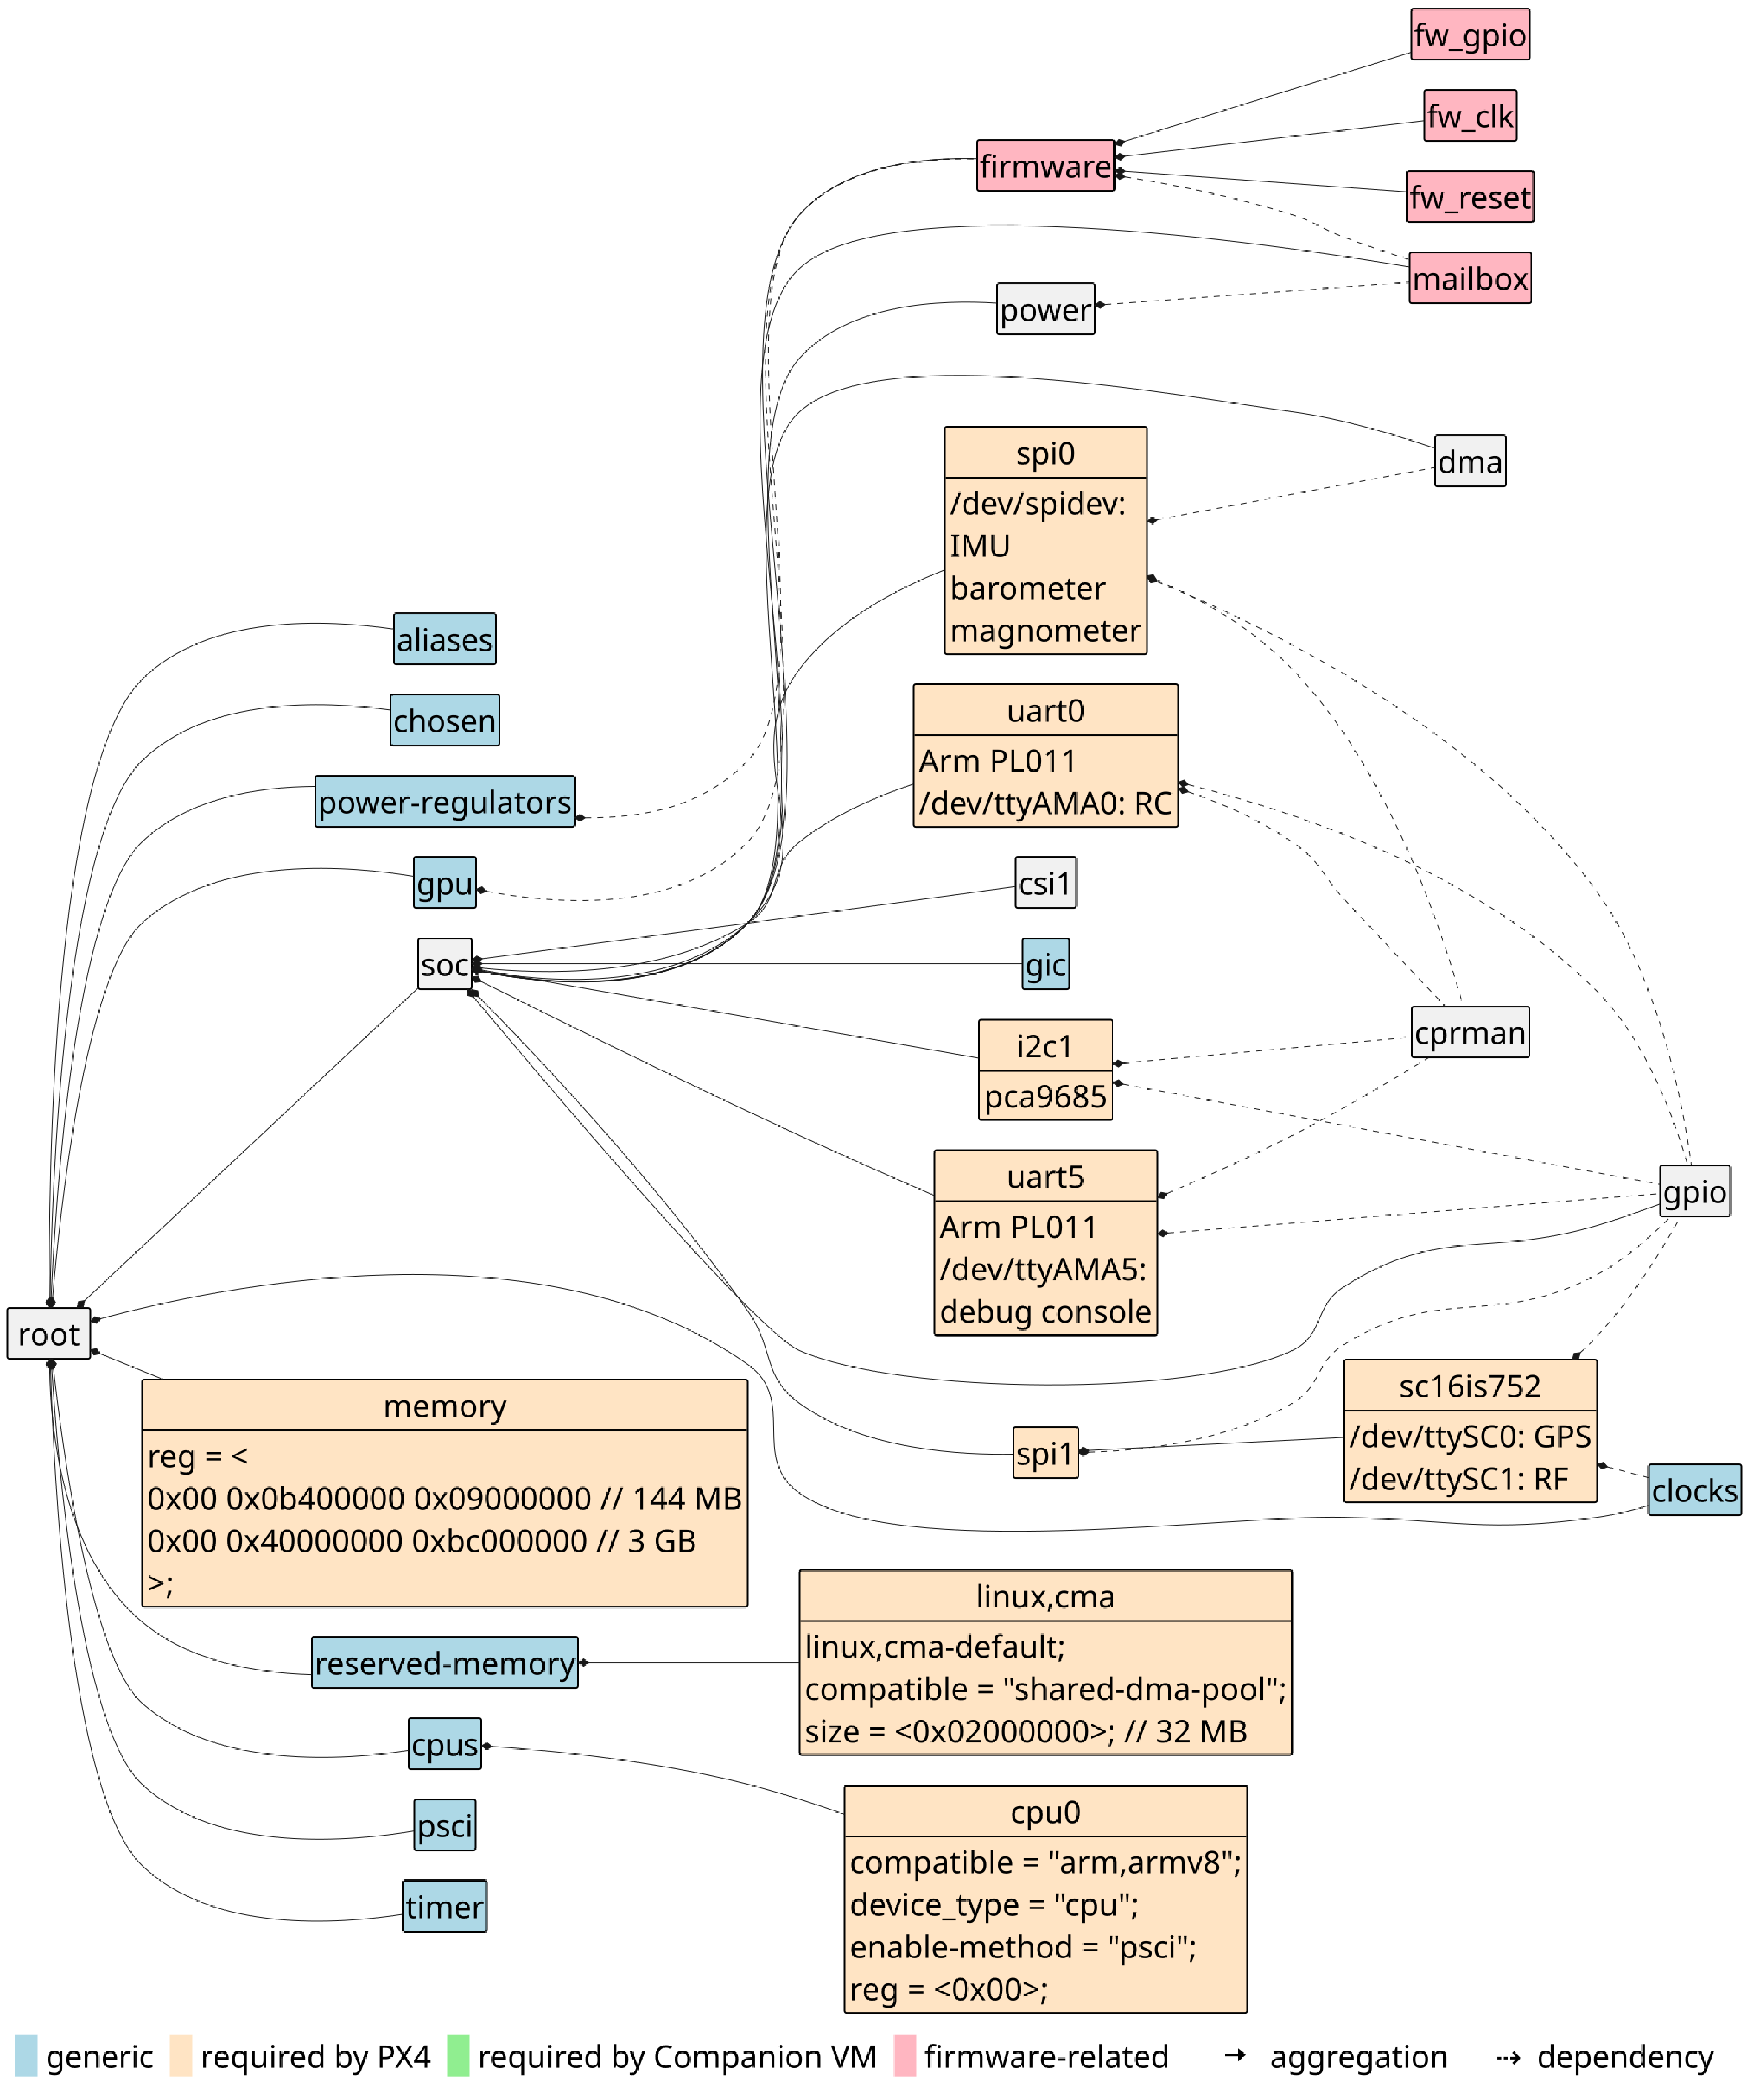
\includegraphics[width=0.85\textwidth]{./img/pdf/hw-map-2}
  \caption[Hardware mapping: SSPFS device tree -- PX4]{Hardware mapping:
  \gls{sspfs} device tree — PX4}%
  \label{fig:hw-map-2}
\end{figure}

\begin{figure}[!hbt]
  \centering
  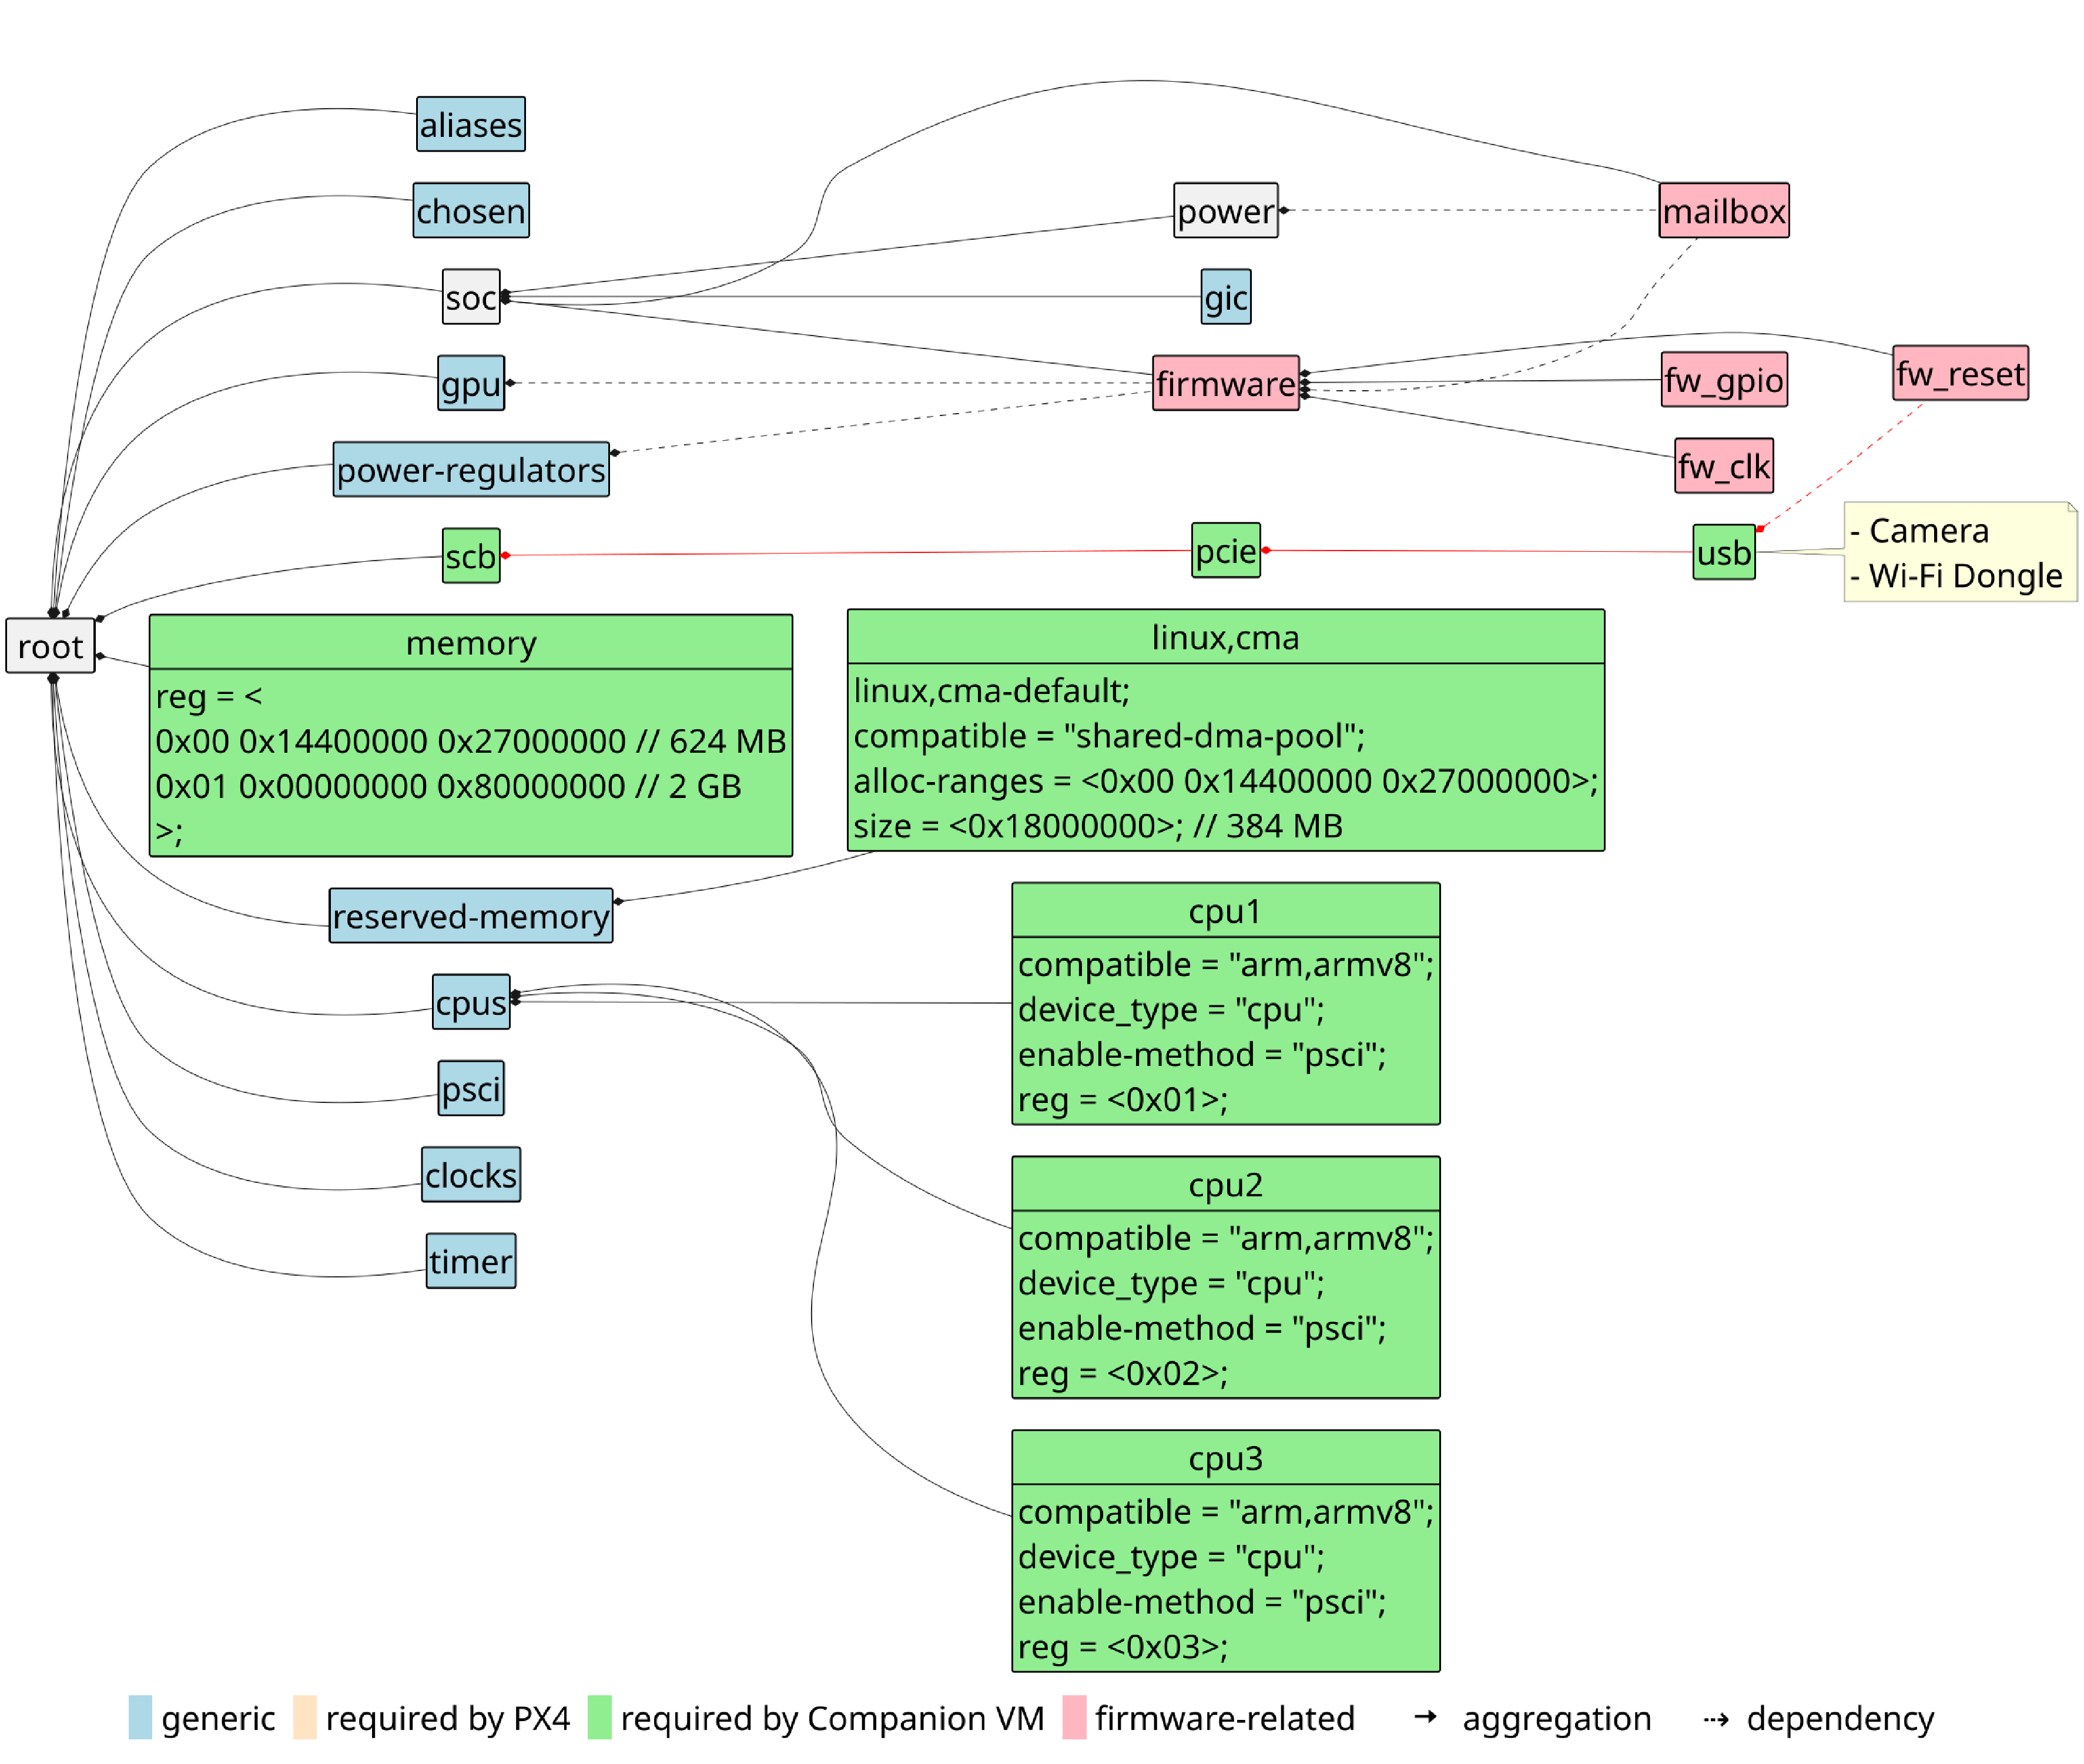
\includegraphics[width=0.85\textwidth]{./img/pdf/hw-map-3}
  \caption[Hardware mapping: SSPFS device tree -- Companion VM]{Hardware
    mapping: \gls{sspfs} device tree — Companion VM}%
  \label{fig:hw-map-3}
\end{figure}

The PX4 \gls{vm} includes only essential onboard
sensors and actuators plus an optional debug console.
Memory is split into two \gls{ram} regions of 144~MB and 3~GB. Within the first region, a 32~MB
\gls{cma} area is reserved to support \gls{dma} transactions for \gls{spi}
devices, which must operate within the first 1~GB of
memory~\cite{bcm2711peripherals}. Processing resources comprise a single Arm A72
\gls{cpu} (core~0).
%
The Companion \gls{vm} exposes the \gls{usb} host for a \gls{usb} camera and a Wi-Fi dongle. Memory allocation features two
\gls{ram} regions of 624~MB and 2~GB. Within the first region, a
384~MB \gls{cma} area supports the video pipeline, which is also restricted to the first 1~GB of
memory~\cite{bcm2711peripherals}. Processing resources comprise three Arm
A72 \glspl{cpu} (cores~1–3).

\subsection{Addons}
\label{sec:addons}
The Companion \gls{vm} requires two \gls{usb} devices: a camera and a Wi-Fi
dongle. Fig.~\ref{fig:addons-cam} shows the selected camera, the Creative Live!
Cam Sync 1080p~V2~\cite{creative-cam}. It is an affordable \gls{usb} device
supporting full~\gls{hd} capture (1920\(\times\)1080 @ 30~\gls{fps}) with dual built-in
microphones. It is plug-and-play on Linux with in-kernel driver support, and its
long cable allows flexible placement on the \gls{uav}.

Fig.~\ref{fig:addons-wifi} shows the selected \gls{usb} Wi-Fi dongle, the EDUP
AX3000. This dual high-gain model offers tri-band support (2.4, 5, and
6~GHz) and data rates up to 3000~\gls{mbps} over a \gls{usb}~3.0 interface~\cite{ax3000-specs}. It uses the Mediatek \lstinline{mt7921au} chipset,
has broad \gls{os} compatibility, and has been supported in-kernel since
Linux~5.18~\cite{ax3000-linux}.

\begin{figure}[!hbt]
  \centering
  % Row 1: Two half-width images
  \begin{subfigure}[t]{0.49\textwidth}
    \centering
    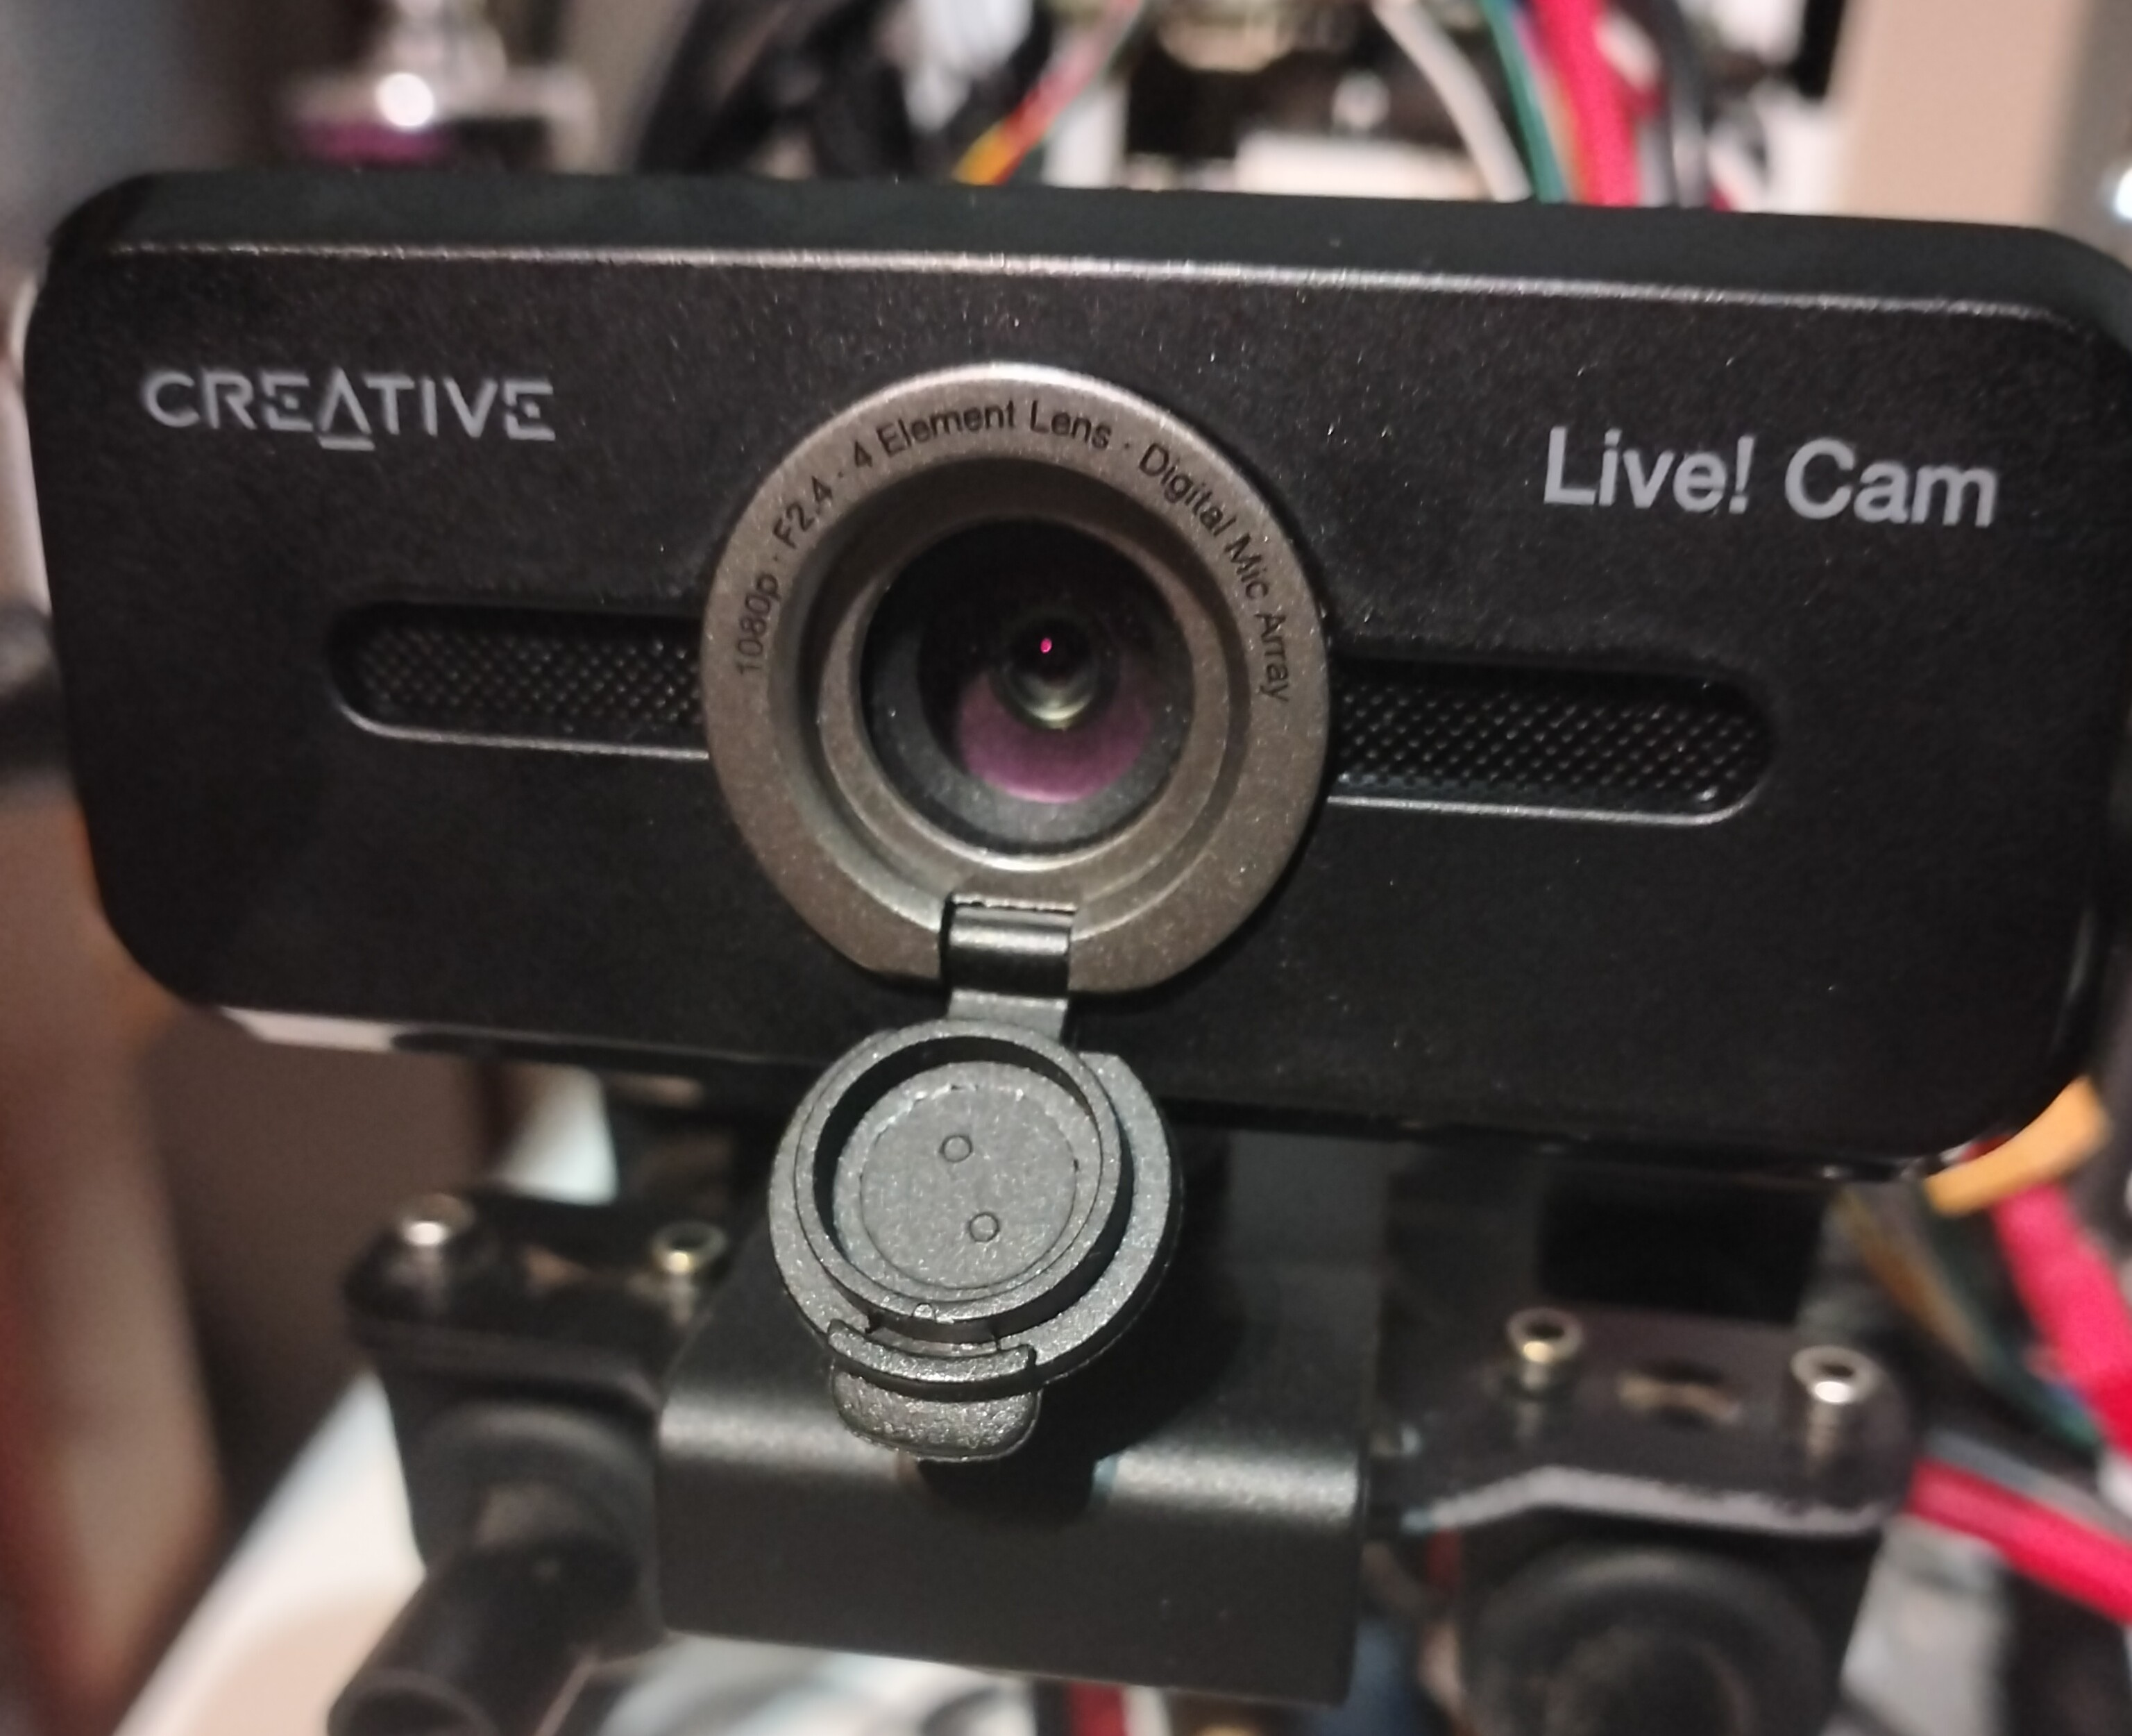
\includegraphics[width=1.0\textwidth]{./img/jpg/creative-cam} 
    \caption{USB Camera -- Creative Live!}%
    \label{fig:addons-cam}
  \end{subfigure}
%  \\[0.5\baselineskip] % Vertical space after first row
  \begin{subfigure}[t]{0.49\textwidth}
    \centering
  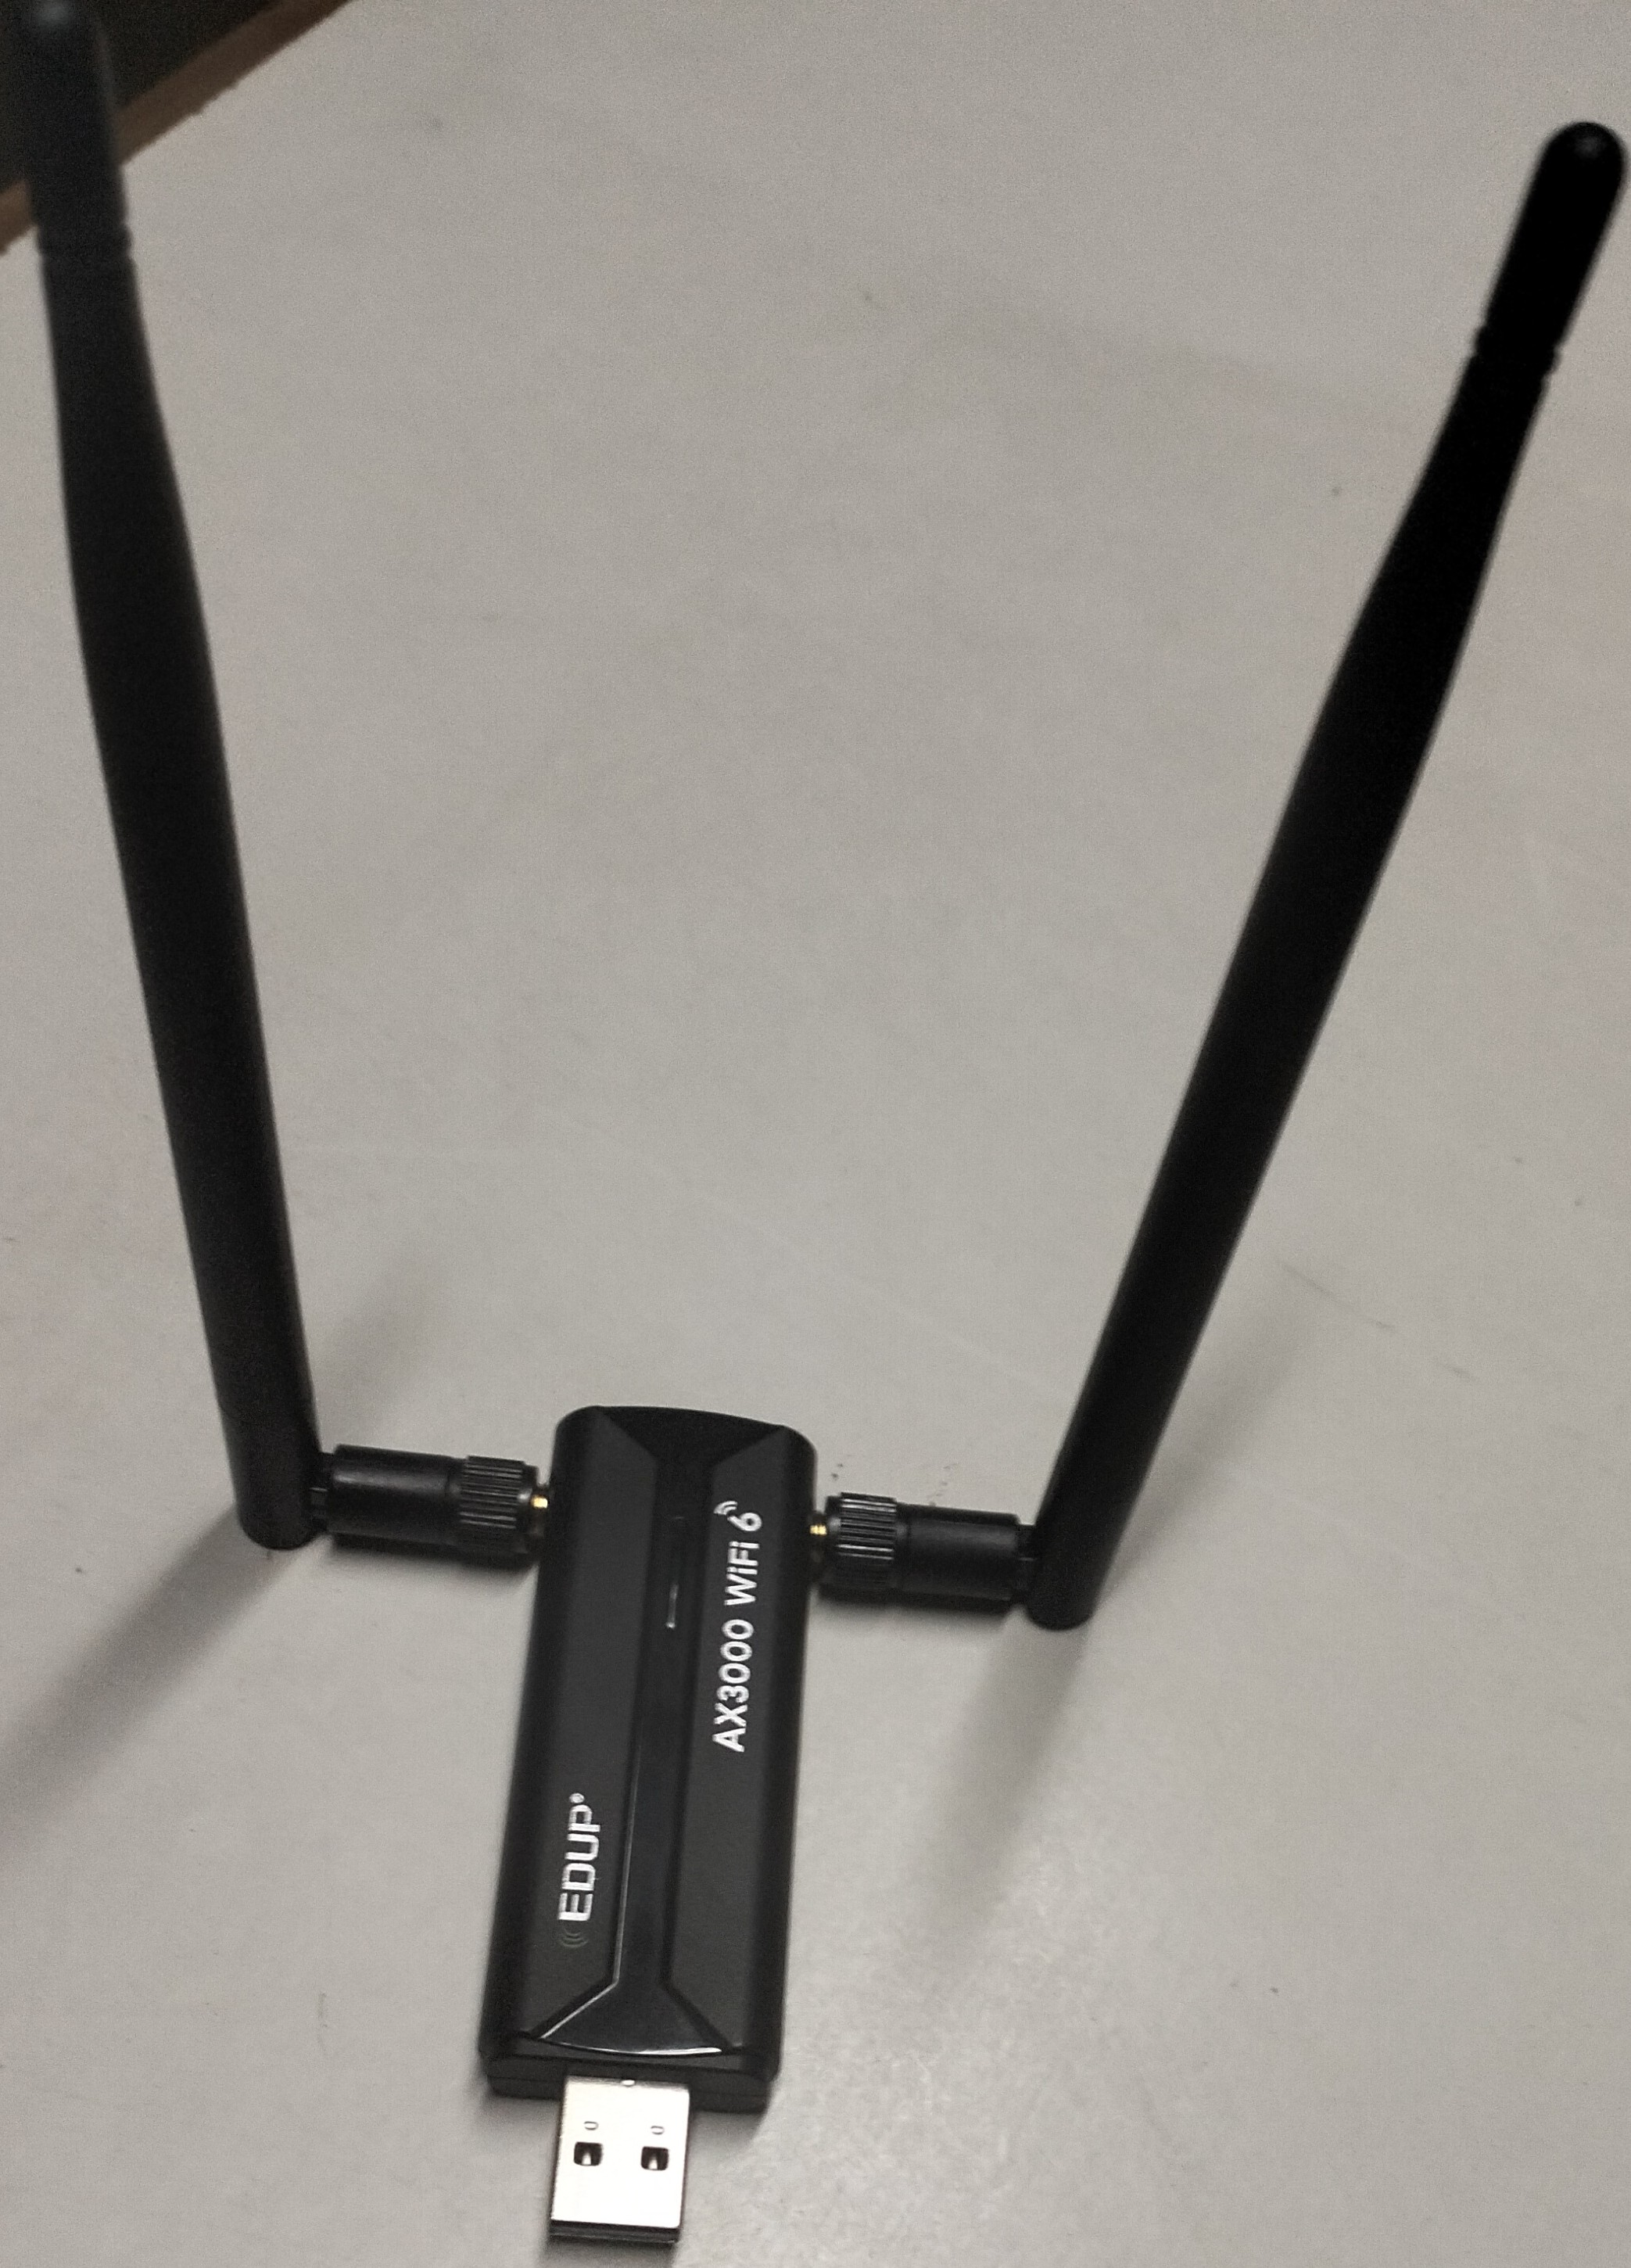
\includegraphics[width=0.6\textwidth]{./img/jpg/ax3000} 
    \caption{USB Wi-Fi dongle -- EDUP AX3000}%
    \label{fig:addons-wifi}
  \end{subfigure}
  \caption{Addons}
  \label{fig:addons}
\end{figure}

%%% Local Variables:
%%% mode: latex
%%% TeX-master: "../template"
%%% reftex-default-bibliography: ("../Bibliography/mieeic.bib")
%%% ispell-local-dictionary: "american"
%%% End:
